\documentclass[a4paper]{article}

%Пакеты для математических символов:

\usepackage{amsmath} % американское математическое сообщество.
\usepackage{amssymb} % миллион разных значков и готический, ажурный шрифты.
\usepackage{amscd} % диаграммы, графики.
\usepackage{amsthm} % окружения теорем, определений и тд.
\usepackage{physics} % основные физические символы
\usepackage{tikz-feynhand} % Феймановские диограммы
%\usepackage{latexsym} % треугольники и пьяная стрелка.

%пакеты для шрифтов:
%\usepackage{euscript} % прописной шрифт с завитушками.
\usepackage{MnSymbol} % Значеки доказательства
\usepackage{verbatim} % улучшенный шрифт "пишущей машинки".
\usepackage{array} % более удобные таблицы.
%\usepackage{multirow} % мультистолбцы в таблицах.
%\usepackage{longtable} % таблицы на несколько страниц.
%\usepackage{latexsym}
\usepackage{collectbox} % Добавляет коробочки, можно складывать туда текст)

\usepackage[backend=biber, style=gost-numeric]{biblatex} % Литература по госту

    
%Пакеты для оформления:
\RequirePackage[center, medium]{titlesec}% Стиль секций и заголовков
%\usepackage[x11names]{xcolor} % 317 новых цветов для текста.
\usepackage{float} % Позволяет использовать H, h! для локации фигур
%\usepackage{multicol} % набор текста в несколько колонн.
\usepackage{graphicx} % расширенные возможности вставки стандартных картинок.
\usepackage{subcaption} % возможность вставлять картинки в строчку
%\usepackage{caption} % возможность подавить нумерацию у caption.
\usepackage{wrapfig} % вставка картинок и таблиц, обтекаемых текстом.
\usepackage{cancel} % значки для сокращения дробей, упрощения, стремления.
\usepackage{misccorr} % в заголовках появляется точка, но при ссылке на них ее нет.
\usepackage{indentfirst} % отступ у первой строки раздела
%\usepackage{showkeys} % показывает label формул над их номером.
%\usepackage{fancyhdr} % удобное создание верхних и нижних колонтитулов.
%\usepackage{titlesec} % еще одно создание верхних и нижних колонтитулов
\usepackage{hyperref} % Ссылки как внешние так и внутренние
\hypersetup{
    colorlinks=true,
    linkcolor=black,
    filecolor=magenta,      
    urlcolor=cyan,
    pdftitle={Overleaf Example},
    pdfpagemode=FullScreen,
    }

    
\usepackage{xcolor} %Позволяет перекрасить все страници
\definecolor{mycolor}{RGB}{244,228,215} %Цвет перекраски


%Пакеты шрифтов, кодировок. НЕ МЕНЯТЬ РАСПОЛОЖЕНИЕ.
\usepackage[utf8]{inputenc} % кодировка символов.
%\usepackage{mathtext} % позволяет использовать русские буквы в формулах. НЕСОВМЕСТИМО С tempora.
\usepackage[T1, T2A]{fontenc} % кодировка шрифта.
\usepackage[english, russian]{babel} % доступные языки.

%tikz:
\usepackage{tikz} % tikz
\usetikzlibrary{decorations.text} % позволяет делать текст вдоль кривой.
\usetikzlibrary{external} % позволяет кэшировать рисунки tikz.


\usepackage{pgfplotstable}

%Отступы и поля:
%размеры страницы А4 11.7x8.3in
\textwidth=7.3in % ширина текста
\textheight=10in % высота текста
\oddsidemargin=-0.5in % левый отступ(базовый 1дюйм + значение)
\topmargin=-0.5in % отступ сверху до колонтитула(базовый 1дюйм + значение)


%Сокращения
%Скобочки
\newcommand{\inrad}[1]{\left( #1 \right)}
\newcommand{\inner}[1]{\left( #1 \right)}
\newcommand{\infig}[1]{\left\{ #1 \right\}}
\newcommand{\insqr}[1]{\left[ #1 \right]}
\newcommand{\ave}[1]{\left\langle #1 \right\rangle}

%% Красивые <= и >=
\renewcommand{\geq}{\geqslant}
\renewcommand{\leq}{\leqslant}

%%Значек выполнятся
\newcommand{\per}{\hookrightarrow}

%%Векторная алгебра
\newcommand{\rot}{\text{rot}}
\renewcommand{\div}{\text{div}}
\renewcommand{\grad}{\text{grad}}

%% Более привычные греческие буквы
\renewcommand{\phi}{\varphi}
\renewcommand{\epsilon}{\varepsilon}
\newcommand{\eps}{\varepsilon}
\newcommand{\com}{\mathbb{C}}
\newcommand{\re}{\mathbb{R}}
\newcommand{\nat}{\mathbb{N}}
\newcommand{\stp}{$\filledmedtriangleleft$}
\newcommand{\enp}{$\filledmedsquare$}

%%Тензорный анализ ОТО теория поля
\newcommand{\Li}[1]{\mathfrak{L}_{#1}}
\newcommand{\crist}[3]{\cfrac{1}{2} \inner{g_{#1#2,#3} + g_{#1#3,#2} - g_{#2#3,#1}}}
\newcommand{\piv}[2]{\cfrac{\partial #1}{\partial #2}}
\newcommand{\llp}[1]{\lambda_{\Lambda_{#1}}}

\newcommand{\redd}[1]{\textcolor{red}{#1}}%Красный текст
\newcommand{\newdot}{\textbullet \hspace{0.5em}}%абзац начинающийся с точки


\makeatletter
\newcommand{\sqbox}{%
    \collectbox{%
        \@tempdima=\dimexpr\width-\totalheight\relax
        \ifdim\@tempdima<\z@
            \fbox{\hbox{\hspace{-.5\@tempdima}\BOXCONTENT\hspace{-.5\@tempdima}}}%
        \else
            \ht\collectedbox=\dimexpr\ht\collectedbox+.5\@tempdima\relax
            \dp\collectedbox=\dimexpr\dp\collectedbox+.5\@tempdima\relax
            \fbox{\BOXCONTENT}%
        \fi
    }%
}
\makeatother
\newcommand{\mergelines}[2]{
\begin{tabular}{llp{.5\textwidth}}
#1 \\ #2
\end{tabular}
}
\newcommand\tab[1][0.51cm]{\hspace*{#1}}
\newcommand\difh[2]{\frac{\partial #1}{\partial #2}}

\newcounter{customsection}
\newcommand{\mysection}[1]{
    \refstepcounter{customsection}
    \addcontentsline{toc}{section}{Appendix \arabic{customsection}: #1} % Добавляет запись в содержание
    \noindent\textbf{Appendix \arabic{customsection}: #1} % Как выглядит в тексте 
} % Независимые секции (аппендиксы) 

\title{Измерение формфактора полулептонного распада $\Lambda_c$-бариона, на данных Belle.}
\date{15 Октября 2024}

\numberwithin{equation}{section}


\begin{document}

\begin{titlepage}
    \centering
    \vspace*{2cm}  % Добавление отступа сверху

    {\Huge \textbf{Измерение формфактора полулептонного распада $\Lambda_c$-бариона.}} % Название крупным шрифтом

    \vspace{1.5cm}

    \vfill  % Вертикальное выравнивание по центру


    \vspace{1cm}

    15 Октября 2024

    \vspace{2cm}

\end{titlepage}

\newpage
\tableofcontents
\newpagestyle{main}{
\setfootrule{0.4pt}
\setfoot{}{\thepage}{\sectiontitle }}
\pagestyle{main}


\section{Введение}

\subsection{Мотивация}

Предпосылки открытия очарованного бариона $\Lambda_c$ появились в 1975 году, когда в результате наблюдения аномалии в распаде $e^+ e^- \to e^+ + \mu^- + E_{miss}$ (см. \textbf{\cite{PhysRevLett1975}}) было высказано предположение о существовании заряженного лёгкого очарованного бариона. Открытие на достаточном уровне значимости произошло более чем 10 лет спустя на коллайдере SPEAR (см. \textbf{\cite{Avery1988}}) по распаду $\Lambda_c \to p K^- \pi^+$. 

$\Lambda_c$, будучи самым лёгким из очарованных барионов, распадается исключительно посредством слабого взаимодействия, что позволяет изолировать и исследовать вклад этого взаимодействия в барионных системах.
В частности, канал $\Lambda_c \rightarrow \Lambda l \nu_l$, где $l = e, \mu$, а распад с продуктом $l = \tau$ подавлен в силу закона сохранения 4-импульса:

\begin{equation*}
    m_{\Lambda_c} = 2.28646\,\text{GeV} < 2.89261\,\text{GeV} = 1.77693\,\text{GeV} + 1.11568\,\text{GeV} = m_{\tau} + m_{\Lambda}.
\end{equation*}

Бранчинговые отношения для полулептонных распадов $\Lambda_c \rightarrow \Lambda l \nu_l$, где $l = e, \mu$, были измерены в нескольких работах. Для канала $\Lambda_c \rightarrow \Lambda e \nu_e$ измеренное бранчинговое отношение составляет $B(\Lambda_c \rightarrow \Lambda e \nu_e) = 3.56 \pm 0.13\%$, как указано в статье \cite{CLEO2023}. Для канала $\Lambda_c \rightarrow \Lambda \mu \nu_{\mu}$ измеренное бранчинговое отношение равно $B(\Lambda_c \rightarrow \Lambda \mu \nu_{\mu}) = 3.48 \pm 0.17\%$ согласно \cite{CLEO2023}.

Полулептонные распады $\Lambda_c$ являются удобным и относительно простым случаем для исследования переходов тяжелого кварка в лёгкий, что позволяет точнее проверять предсказания теоретических моделей, таких как эффективная теория тяжёлых кварков (HQET) и квантовая хромодинамика на решётке (LQCD). Проверка этих моделей с помощью экспериментов может не только подтвердить их верность, но и выявить отклонения от стандартной модели, что потенциально указывает на существование новой физики, включая новые взаимодействия или экзотические частицы.

\subsection{Отличие от работы CLEO}

Измерение форм-фактора $\Lambda_c \rightarrow \Lambda l \nu_l$ важно для проверки результатов предыдущего эксперимента \textbf{\cite{CLEO2023}}, в котором был измерен форм-фактор $\Lambda_c \rightarrow \Lambda e \nu_e$. Важно сравнить методологические и экспериментальные аспекты текущего исследования с работой команды CLEO.

Прежде всего, команда CLEO сделала предположение о том, что спин бариона $\Lambda$ равномерно распределён. Это предположение оказывает влияние на значение спиральности, которое напрямую входит в уравнение для форм-фактора. В данной работе предлагается более точное измерение распределения направлений спина, основанное на анализе распада в канале $\Lambda_c^+ \rightarrow \Lambda \pi^+$. Этот подход позволяет уменьшить систематические ошибки и повысить точность вычислений.

Второе важное отличие заключается в использовании независимого источника данных. В то время как команда CLEO использовала данные, собранные с детектора "CLEO" на Корнельском электронном накопительном кольце (Cornell Electron Storage Ring), в настоящей работе анализ проводился на детекторе "Belle", установленном на ускорителе "KEK". Это не только обеспечивает независимую проверку результатов, но и позволяет уточнить их с учётом различий в экспериментальных установках.

Наконец, команда CLEO не проводила анализа полулептонного распада $\Lambda_c \rightarrow \Lambda \mu \nu_\mu$, что является существенным упущением. В данном исследовании этот канал был тщательно изучен, что позволяет расширить понимание полулептонных распадов и улучшить тесты на универсальность лептонов.

Таким образом, данная работа вносит вклад в дальнейшее изучение свойств бариона $\Lambda_c$ и уточнение результатов, полученных в предыдущих исследованиях.

\subsection{Модели и теоретические предсказания}

Как уже было сказано выше, на данный момент существуют численные методы вычисления форм-факторов, основанные на различных приближениях или моделях. Все они дают различные результаты (см. таблицу \ref{tb:chd}). Поскольку сильное взаимодействие сложно поддаётся теоретическим расчётам из-за отсутствия малого параметра, результаты могут быть проверены только экспериментально.

\begin{table}[H]
    \centering
    \caption{Форм-факторы полулептонных распадов $\Lambda_c \to \Lambda$ для $q^2 = 0$.}
    \begin{tabular}{|c|c|c|c|c|c|c|}
    \hline
    Form Factor & $\mathfrak{F}_1^V(0)$ & $\mathfrak{F}_2^V(0)$ & $\mathfrak{F}_3^V(0)$ & $\mathfrak{F}_1^A(0)$ & $\mathfrak{F}_2^A(0)$ & $\mathfrak{F}_3^A(0)$ \\
    \hline
    \textbf{\cite{QCD2021}} & 0.687(138) & 0.486(117) & 0.164(80) & 0.539(101) & -0.388(100) & -0.359(283) \\
    \hline
    \textbf{\cite{BagModel1989}} & 0.35 & 0.09 & 0.25 & 0.61 & -0.04 & -0.11 \\
    \hline
    \textbf{\cite{RQM2016}} & 1.14 & 0.072 & 0.252 & 0.517 & -0.697 & -0.471 \\
    \hline
    \textbf{\cite{QSR2009}} & 0.665 & 0.285 & --- & 0.665 & -0.285 & --- \\
    \hline
    \textbf{\cite{LFCQM2018}} & 0.468 & 0.222 & --- & 0.407 & -0.035 & --- \\
    \hline
    \end{tabular}
    \label{tb:chd}
\end{table}


\section{Экспериментальная установка}

\subsection{Коллайдер KEK}
Ускоритель KEKB является электрон-позитронным коллайдером, состоящим из двух 
колец, пересекающихся в одной точке под углом $22\,\text{mrad}$, что позволяет измерять CP-асимметрию. 
Пучки электронов и позитронов сталкиваются с энергией $8\,\text{GeV}$ и $3.5\,\text{GeV}$ соответственно.
Пучки рождаются на фотонной фабрике и, проходя через линейный ускоритель, где разгоняются до скорости, близкой к скорости света, 
передаются в основные кольца. В режиме накопления пучка подача происходит непрерывно, а в нормальном режиме 
сбора данных - периодически, раз в несколько миллисекунд.

Основной целью было производство большого количества B-мезонов. Работа ускорителя началась в декабре
1998 года и закончилась в конце июня 2010 года. За это время KEKB установил мировой
рекорд по светимости - $2.11\times 10^{34} cm^{-2}s^{-1}$, который на сегодняшний день был
превзойдён только на коллайдере SuperKEKB - усовершенствованной версии, собранной
на основе KEKB. За все время было собрано $825.547fb^{-1}$.

\begin{figure}[H]
    \centering
    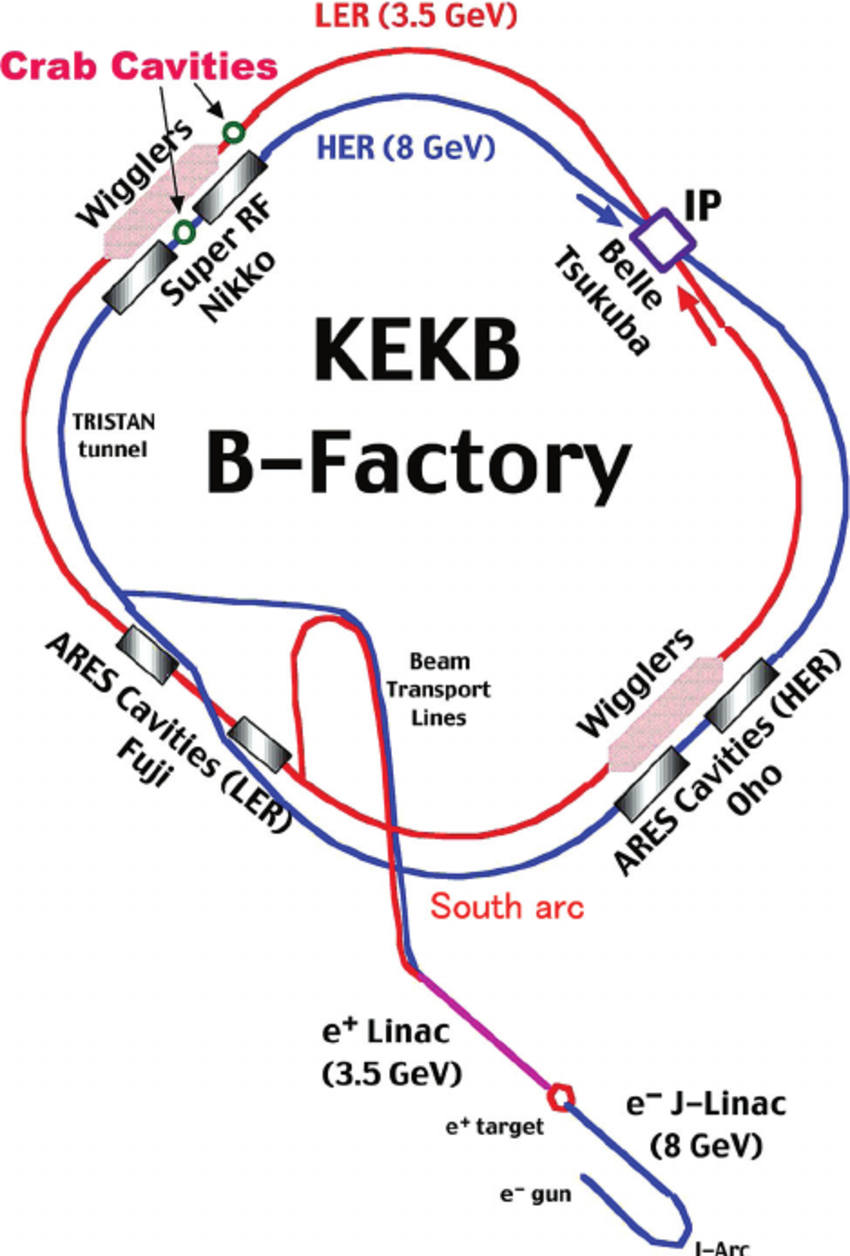
\includegraphics[width=0.5\linewidth]{img/kekb.png}
    \caption{Ускорительный комплекс KEKB}
    \label{the:kek}
\end{figure}

\subsection{Детектор Belle}

Детектор Belle охватывал весь азимутальный угол, а также перекрывал 
часть полярного угла от $17^{\circ} $ до $150^{\circ} $, что соответствует $0.74$
полного телесного угла. Установка окружала точку взаимодействия и состояла 
из вершинного кремниевого детектора (SVD), центральной дрейфовой 
камеры (CDC) из 50 цилиндрических слоёв, массива аэрогелевых черенковских 
счётчиков (ACC), системы измерения времени пролёта (TOF) из сцинтилляционных 
счётчиков, электромагнитного калориметра (ECL), изготовленного из кристалов 
йодида цезия (CsI), и переднего калориметра (EFC), расположенных внутри 
сверхпроводящего соленоида, обеспечивающего магнитное поле величиной 
$1.5 Tl$. В железном ярме электромагнита был расположен детектор $K_L^0$ мезонов 
и $\mu$ (KLM), составленный из стеклянных резистивных плоских камер. 
Общий вид детектора Belle показан на рис. \ref{the:belle}. Подробно о поддетекорах 
и востановлении события в \redd{ссылка на аппендикс}.

\begin{figure}[H]
    \centering
    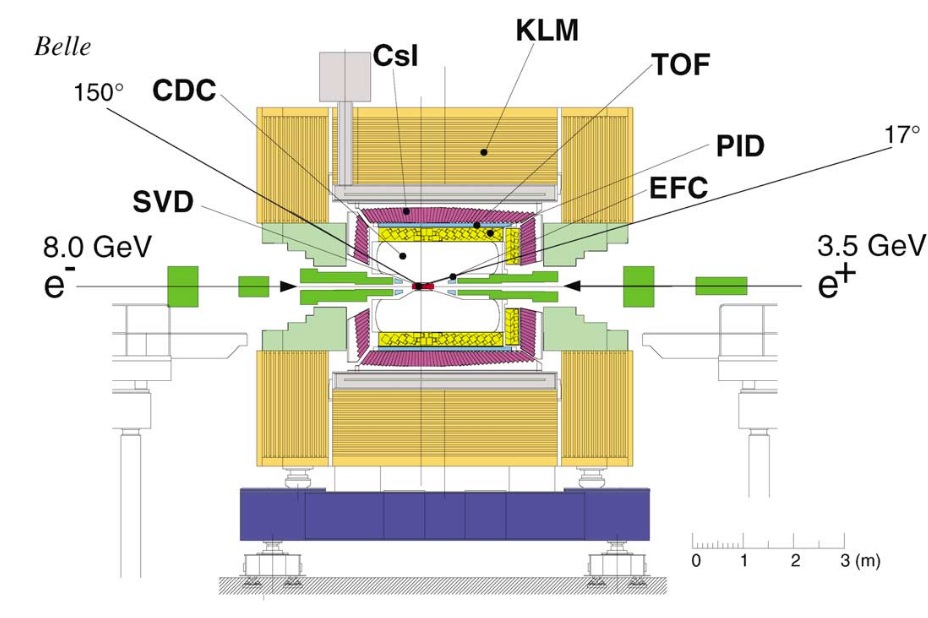
\includegraphics[width=0.8\linewidth]{img/the_belle.png}
    \caption{Декткор Belle в сечении}
    \label{the:belle}
\end{figure}





\section{Методы измерения}
\subsection{SVD}

\begin{wrapfigure}{r}{0.5\textwidth}
    \centering
    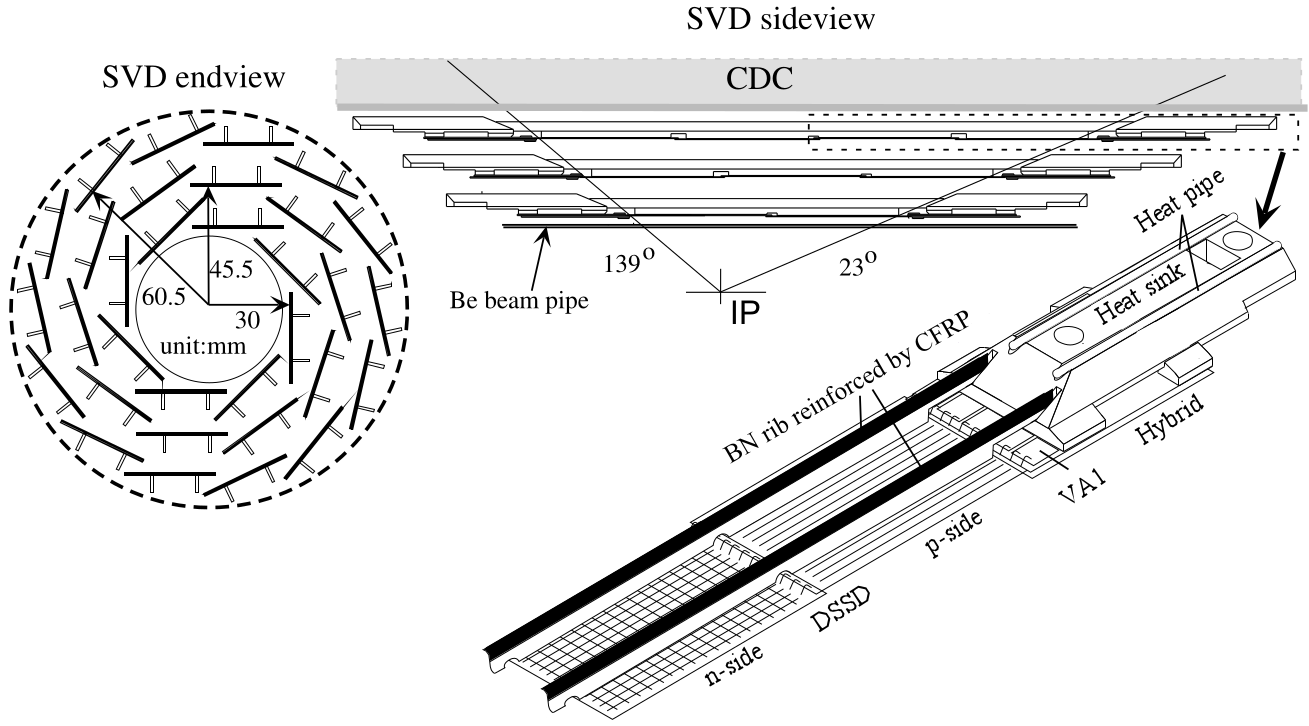
\includegraphics[width=0.48\textwidth]{img/SVD.png}
    \caption{Схематическое изображение SVD.}
    \label{the:SVD}
\end{wrapfigure}

Кремниевый вершинный детектор (рис. \ref{the:SVD}), расположенный непосредственно у точки взаимодействия, 
служит для определения её точного местоположения. Он состоит из тонких слоёв, охватывающих угловой диапазон от $23^\circ$ до $139^\circ$, 
расположенных внахлёст и разделённых на секции, в которых при пролёте частиц 
образуются электронно-дырочные пары. Благодаря большому сечению взаимодействия, 
высокой плотности материала и низкой энергии взаимодействия, полупроводниковые 
детекторы обладают высокой точностью при измерении широкого диапазона энергий частиц.
Это позволяет определять точку взаимодействия с точностью до 100 мкм. 
Однако, несмотря на значительно более высокую точность по сравнению с газовыми детекторами, 
монтаж большого количества слоёв усложнён из-за возможных сильных отклонений 
трека в результате многократного взаимодействия с плотными кристаллами кремния.

\subsection{Система идентификации заряженных адронов}

Система включает в себя три основные детектора: CDC, TOF и ACC.

\begin{wrapfigure}{r}{0.5\textwidth}
    \centering
    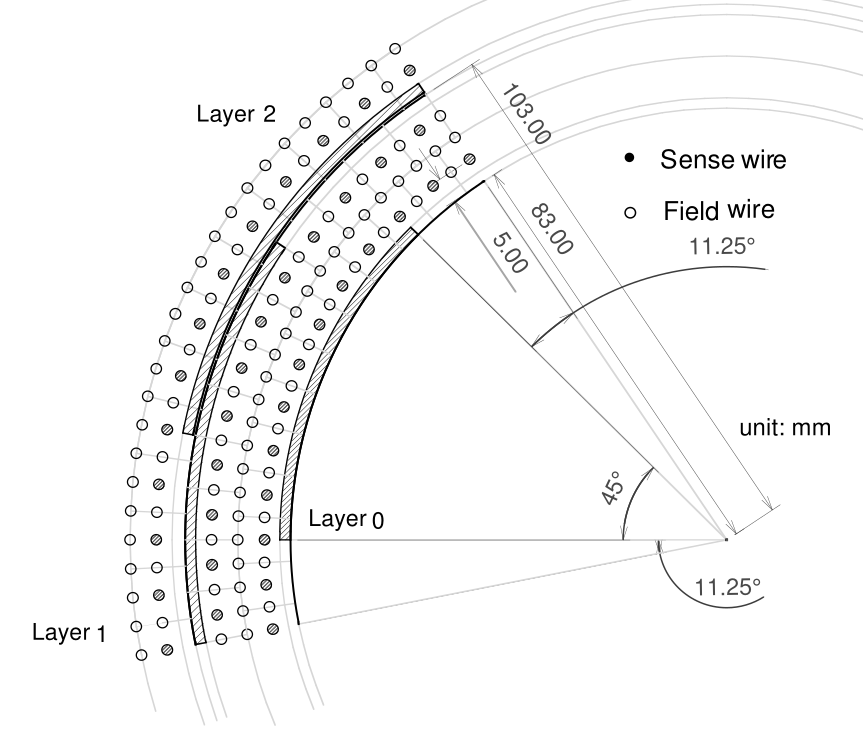
\includegraphics[width=0.3\textwidth]{img/CDC.png}
    \caption{Конфигурация слоёв проволок в центральной дрейфовой камере (CDC).}
    \label{the:CDC}
\end{wrapfigure}

CDC (центральная дрейфовая камера) представляет собой вытянутый цилиндр, слегка деформированный для 
эффективного охвата полярного угла от $17^\circ$ до $150^\circ$. Камера заполнена смесью газов $He$ и $C_2H_6$, 
что минимизирует влияние на трек частицы и обеспечивает максимальную эффективность ионизации. 
Высвобождающиеся электроны движутся к тонким алюминиевым проволокам, натянутым внутри объёма CDC (рис. \ref{the:CDC}). 
На проволоки подаётся напряжение порядка $20$ кВ/см. При достижении электронами проволок происходит лавинное умножение электронов, 
что фиксируется системой. Вся камера находится в магнитном поле с индукцией около $1.5$ Тл, что позволяет измерять импульс 
частицы по кривизне её трека. Также потери энергии на ионизацию позволяют оценить массу частицы, что, в свою очередь, 
помогает в идентификации заряженных частиц.

\begin{wrapfigure}{l}{0.5\textwidth}
    \centering
    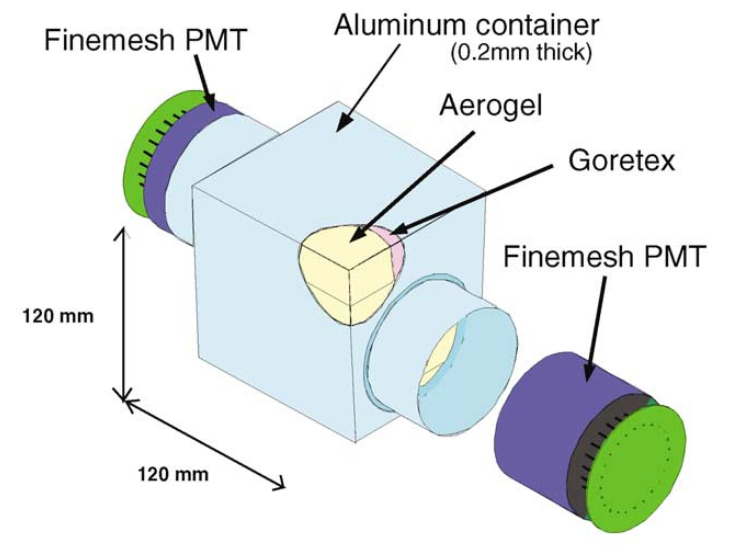
\includegraphics[width=0.4\textwidth]{img/ACC.png}
    \caption{Детектор черенковского излучения (ACC).}
    \label{the:ACC}
\end{wrapfigure}

ACC (детектор черенковского излучения) состоит из отдельных модулей размером $12\times12\times12$ см, 
расположенных цилиндрически и разделённых на 240, 240 и 360 модулей, ориентированных под различными углами для эффективного 
захвата частиц. Дополнительно имеется 228 счётчиков, установленных на торцевой стороне для учёта частиц, движущихся в 
определённом направлении из-за особенностей распределения импульса. Частицы, пролетающие через арогелевые среды, заполняющие 
модули ACC, возбуждают фотоны, длина волны которых зависит от заряда, импульса и массы частицы.

TOF (времяпролётный детектор) — это система пластиковых сцинтилляционных счётчиков, 
направленных на точку взаимодействия, предназначенная для разделения каонов и пионов при импульсах менее $1.2$ ГэВ. 
Такое разделение основано на принципе работы: отклик в 128 сцинтилляционных счётчиках сравнивается с длиной трека, рассчитанной путём 
экстраполяции из трековой системы.


\begin{figure}[!htb]
    \centering
    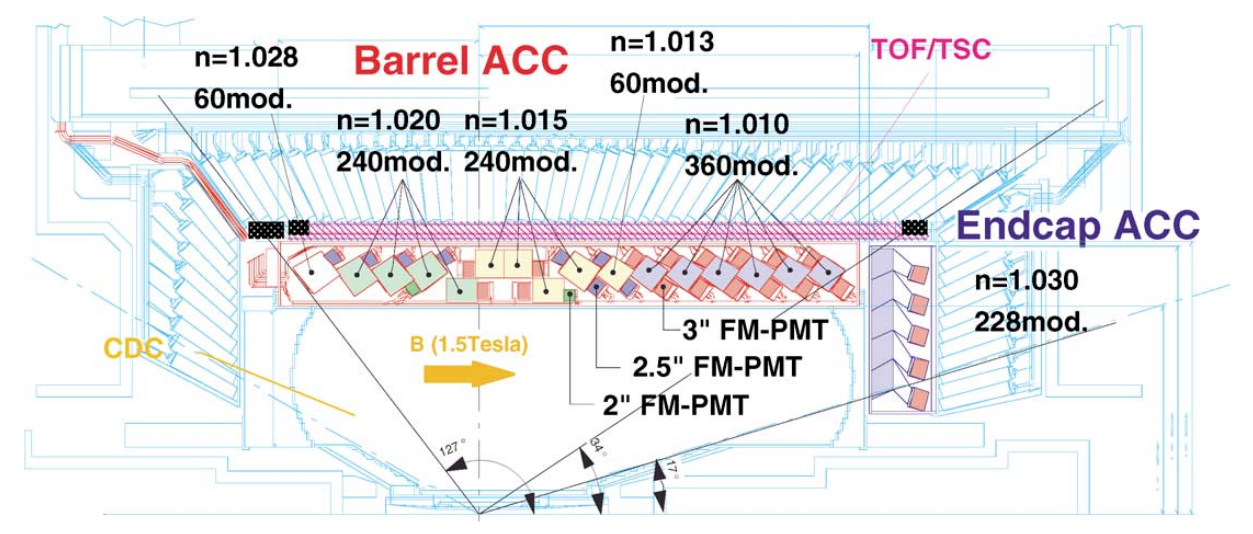
\includegraphics[width=1\linewidth]{img/Ch_hadr_id.png}
    \caption{Полная система идентификации заряженных частиц (ACC, CDC и TOF).}
    \label{the:ch_hadr_id}
\end{figure}

\begin{wrapfigure}{r}{0.5\textwidth}
    \centering
    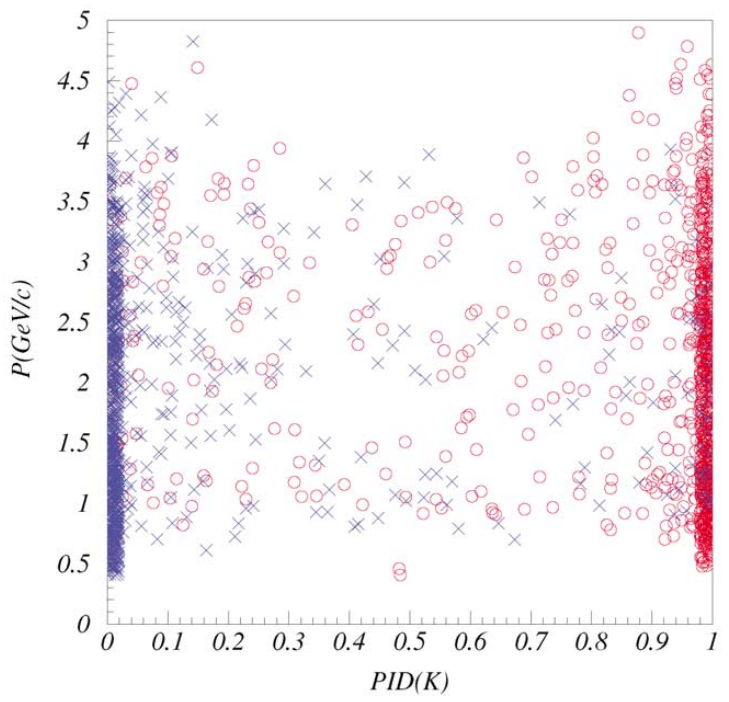
\includegraphics[width=0.7\linewidth]{img/L_P.png}
    \caption{Рапределение $PID$ для $K$ - синие кресты и $\pi$ - красные окружности}
    \label{the:li}
\end{wrapfigure}

На основе данных ACC, CDC и TOF, вычисляются вероятности идентификации частиц для каждого детектора: $L_{ACC}(p)$ для ACC, 
$L_{TOF}(p)$ для TOF и $L_{CDC}(p)$ для CDC, где $p$ — это гипотеза о типе частицы. 
Общая функция правдоподобия рассчитывается как произведение отдельных функций 
$L(p) = L_{ACC}(p) \cdot L_{TOF}(p) \cdot L_{CDC}(p)$.
Затем для двух гипотез о типе частицы вычисляется показатель $PID$ (отношение правдоподобий):
\begin{equation}
    \mathfrak{L}_{a/b} = \frac{L(a)}{L(a) + L(b)},
\end{equation}
где $a$ и $b$ — два возможных типа частицы.






\section{Каналов тагирования}
\label{taging}
\subsection{Тагирование $\Lambda_c$}

Для восстановления распадов $\Lambda_c$-барионов и определения импульса недетектируемого нейтрино применяется тагирование по заряду, аромату и барионному числу. Будем предполагать, что $\Lambda_c$ образуется из $\bar{c}$-кварка и подхваченных из вакуума недостающих кварков. В таком случае будем называть систему центромасс $c$-кварка $X_c$, то есть неизвестная очарованная частица, которая фактически может быть не одной, а несколькими частицами сразу.

\begin{figure}[h!]
    \centering
    \begin{tikzpicture}
        \begin{feynhand}
            \vertex [particle] (e) at (-2,1) {$e^-$};
            \vertex [particle] (ae) at (-2,-1) {$e^+$};
            
            \vertex [particle] (photon) at (0,0);
            \vertex (w1) at (1, 0);
            
            \vertex [particle] (c) at (3,1) {$c$};
            \vertex [particle] (anti_c) at (3,-1) {$\bar{c}$};
        
            \propag [fermion] (e) to (photon);
            \propag [anti fermion] (ae) to (photon);
            \propag [photon] (photon) to  [edge label=$\gamma*$]  (w1);
            \propag [fermion] (w1) to (c);
            \propag [anti fermion] (w1) to (anti_c);
        \end{feynhand}
    \end{tikzpicture}
\end{figure}

Для того чтобы определить состав $X_c$, необходимо, чтобы соблюдались законы 
сохранения барионного числа, аромата, заряда, а также 4-импульса. Такая 
технология называется тагированием \textcolor{red}{ссылка на работу}. В 
результате получим, что в $X_c$ будет входить хотя бы один барион и кварки 
$u c d$, а также любые пары $q \bar{q}$. В итоге возможны следующие варианты 
$X_c$. Также важно понимать, что чем больше частиц содержит $X_c$, тем менее 
вероятно событие с такой комбинацией, так как новые частицы требуют 
дополнительных кварковых пар, создание которых требует больше энергии. 
Кроме того, при добавлении новых частиц время работы программы увеличивается 
экспоненциально, так как сложность алгоритма $\mathcal{O}(\prod_n N_n)$ 
(где $N_n$ количестов задетектированных частиц типа $n$ в событии).

В работе рассматриваются $X_c \to \Lambda^{tag}_c; \Lambda^{tag}_c \pi^- \pi^-; \Lambda^{tag}_c \pi^+ \pi^- \pi^+ \pi^-; D^0 p; D^+ p \pi^-; D*^0 p; D*^+ p \pi^- $, 
чтобы отличать $\Lambda_c$ котрую тагируемую от тагирующей (той что является продуктом $X_c$), вторую обозначаим как $\Lambda^{tag}_c$.
Каналы распада прочих частиц будем импользовать заведомо изветные самые эффективные каналы, согласно \cite{PDGTablesBar} для барионов и \cite{PDGTablesMes} для мезонов.
\begin{figure}[h]
    \centering
    \begin{tabular}{c|c}
        Particle & Channels \\ \hline
        $D^0$ & $K^- \pi^+; K^- \pi^+ \pi^+ \pi^-; K^- K^+; K^0_s \pi^+ \pi^+; K^0_s \pi^0; K^+ K^- K_s^0$ \\
        $D^+$ & $K^- \pi^+ \pi^+; K^0_s; K^0_s \pi^+ \pi^+ \pi^-; K^+ K^- \pi^+$ \\
        $\Lambda^{tag}_c$ & $pK^-\pi^+; \Lambda^0 \pi^+; \Lambda^0 \pi^+ \pi^0; p K_s^0 \pi^0$ \\
        $D*^+$ & $D^0 \pi^0; D^0 \gamma$ \\
        $D*^+$ & $D^+ \pi^0; D^0 \pi^+$ \\
        $\pi^0$ & $\gamma \gamma$ \\
        $K_s^0$ & $\pi^+ \pi^-$
    \end{tabular}
    \label{fig:part_channels}
\end{figure}

\subsection{Критерии отбора}

В данном разделе изложены критерии отбора, принятые на основании работы \cite*{BelleDetector2002} и описанном в \ref{mes_mthods}. 
Имея на набор треков и их параметров, надо их классифицировать по типу частици оставившей этот трек. 

\newdot Фотоны классифицированы, но используемые при реконструкции событий, наложим дополнительное ограничение $E_\gamma > 50 \text{ MeV}$, поскольку фотоны с меньшей энергией трудно отличимы тормозных или индуцированных в сичтеме токов, 
что может привести к ошибочной интерпретации их как сигнальных фотонов.

\newdot Идентификация частиц по (PID):

Как уже известно для треков формируется значение правдоподобия $L(p,a)$ 
и в поледствии PID значение $\mathfrak{L}_{p_1/p_2}(a)$, поэтому на треки котрые хотим 
идентифицировать как частицу $p$ наложим следующие ограничения:

\begin{figure}[h]
    \centering
    \begin{tabular}{c|c}
        Гипотеза & Критекрий \\ \hline
        $p \& \bar p$ & $\mathfrak{L}_{p/K} < 0.6; \mathfrak{L}_{p/\pi} > 0.6$ \\
        $K^\pm$   & $\mathfrak{L}_{p/K} < 0.4; \mathfrak{L}_{K/\pi} > 0.6$ \\
        $\pi^{\pm}$ & все заряженные треки, не прошедшие идентификацию по вышеуказанным критериям \\
    \end{tabular}
\end{figure}

\newdot $K_s^0$-мезоны реконструируются по распаду $K_s^0 \to \pi^+ \pi^-$ из кандидатов, отобранных с помощью стандартного инструмента V0finder и собранных в таблице MdstVee2. Критерии отбора следующие:

$$
\left| M_{K_s^0} - M^{real}_{K_s^0} \right| < 30 \text{ MeV}; \ \rho_{K_s^0} > 1 \text{ мм}; \ z_{K_s^0} > 1 \text{ см}; \ \cos \theta_{K_s^0} > 0.99
$$

где $M^{real}_{K_s^0} = 497.611 \text{ MeV}$, $M_{K_s^0}$ — инвариантная масса пионов ($\pi^+ \pi^-$), собранных в $K_s^0$-мезон, $z_{K_s^0}$ и $\rho_{K_s^0}$ — цилиндрические координаты реконструированной вершины распада $K_s^0$-мезона в лабораторной системе отсчёта, а $\cos \theta_{K_s^0}$ — азимутальный угол между импульсом $K_s^0$ и направлением на его вершину распада.

\newdot $\pi^0$ -мезоны восстанавливались в распаде на два фотона, которые в
свою очередь реконструировались по кластерам энерговыделения в ECL.
Критерии отбора:
$$
\abs{M_{\pi^0} - M_{\pi^0}^{real}} < 15 MeV 
$$
После отбора стандартно были установлены погрешности для импульсов фотонов и выполнены фиты в вершину и массу.

\newdot Отбор $D$ -мезонов:

\begin{figure}[h]
    \centering
    \begin{tabular}{c|c}
        $D^0$ & $\abs{M_{D^0} - M^{real}_{D^0}} < 15 MeV$ \\
        $D^\pm$ & $\abs{M_{D^\pm} - M^{real}_{D^\pm}} < 15 MeV$ \\
        $D*^{\pm}$ & $\abs{M_{D*^\pm} - M^{real}_{D*^\pm}} < 3 MeV$ \\
        $D*^0$ & $\abs{M_{D*^0} - M^{real}_{D*^0}} < 3 MeV$ \\
    \end{tabular}
\end{figure}

Где $M^{real}_{D^\pm} = 1864.83 MeV; M^{real}_{D^0} = 1869.65 MeV; 
M^{real}_{D*^\pm} = 2010.26;  M^{real}_{D*^0} = 2006.85 MeV$. 
Так де на $D*$-мезоны накладываем ограничение:

\begin{equation}
        \abs{M_{D*} - M^d_{D}} < 15 MeV
\end{equation}

Где $ M^d_{D}$ --- масса $D$-мезона используемого для кобинации соответствующего. 
$D^*$. Так как ошибка собранного $D*$ мезона карелирует с собранным 
предврительно $D$-мезоном.



\section{Исследование природы фона и выделение сигнала}

Для исследования природы фона были использованы события, сгенерированные методом Монте-Карло. Для соответствия отобранным данным критерии отбора были выбраны аналогичными. Также была выполнена дополнительная операция — фитирование по массе и по вершине.

Среди множества идентифицированных дочерних продуктов распада частицы $\xi$ можно использовать известные свойства импульсов этих продуктов, исходящих из вершины распада, для корректировки измеренных импульсов. Это позволяет улучшить точность, соответствуя гипотезе (далее этот метод будет называться «фитом в вершину»). Аналогично, исходя из известной инвариантной массы для $\xi$, импульсы дочерних частиц могут быть скорректированы так, чтобы $M_p = \sqrt{\sum_n \inner{p_n}_\gamma \inner{p_n}^\gamma}$ совпадала с $M^{\text{real}}_{\xi}$, где $p_n$ — 4-импульс, соответствующий $d_n$. Этот метод будет называться «фитом в массу». Для этих целей использовались алгоритмы фита в вершину и массу, принятые в коллаборации KEK.

В результате отбора было получено распределение восстановленной массы $\Lambda_c$ (рис. \ref{MC_inc_ful}).

\begin{figure}[H]
    \centering
    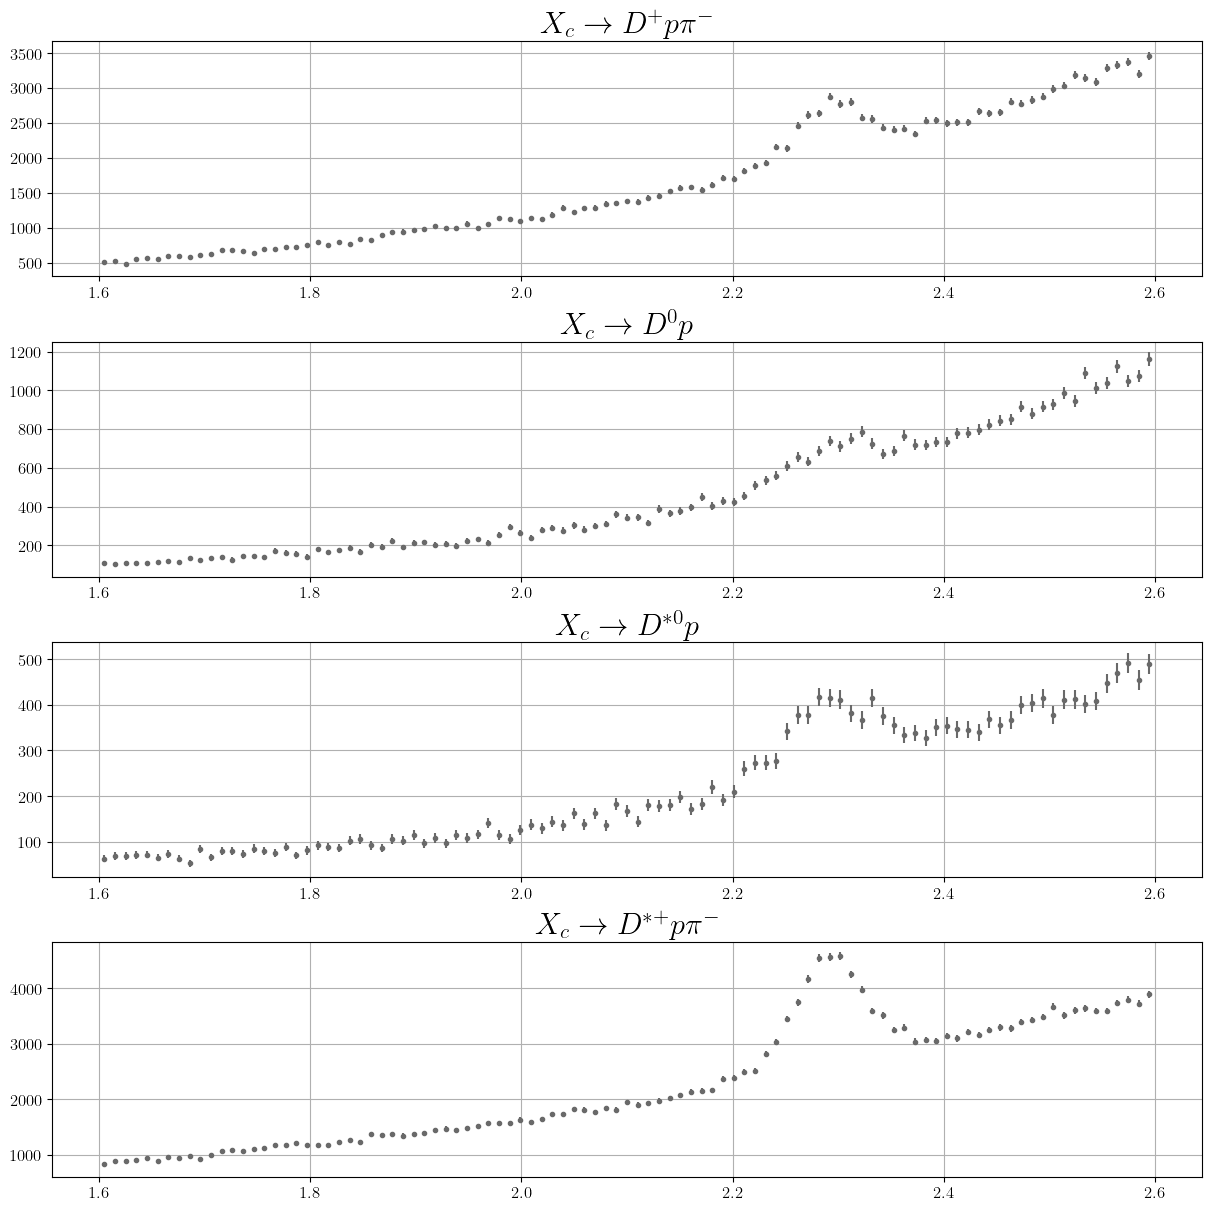
\includegraphics[width=1\linewidth]{img/MC_inc.png}
    \caption{Распределение количества событий по каналам.}
    \label{MC_inc_ful}
\end{figure}

Также в этих событиях была выделена энергия $\Lambda_c$ (если она присутствует); если нет, то $E_{\Lambda_c} = 0$ соответственно.

Для выделения сигнальных событий проводится проверка:

\begin{itemize}
    \item Каждая детектируемая частица правильно идентифицирована, то есть треку была присвоена верная гипотеза на основе информации из Монте-Карло.
    \item $\abs{E_{\text{beam}} - E_{X_c} - E_{\Lambda_c}} < 0.015$ ГэВ, где $E_{\text{beam}}$ — энергия пучков.
    \item Проверяется, что каждая комбинированная частица действительно существовала и распалась по предполагаемому каналу, а дочерние частицы правильно присвоены.
\end{itemize}

В итоге получаем распределение (рис. \ref{MC_sig}).

\begin{figure}[H]
    \centering
    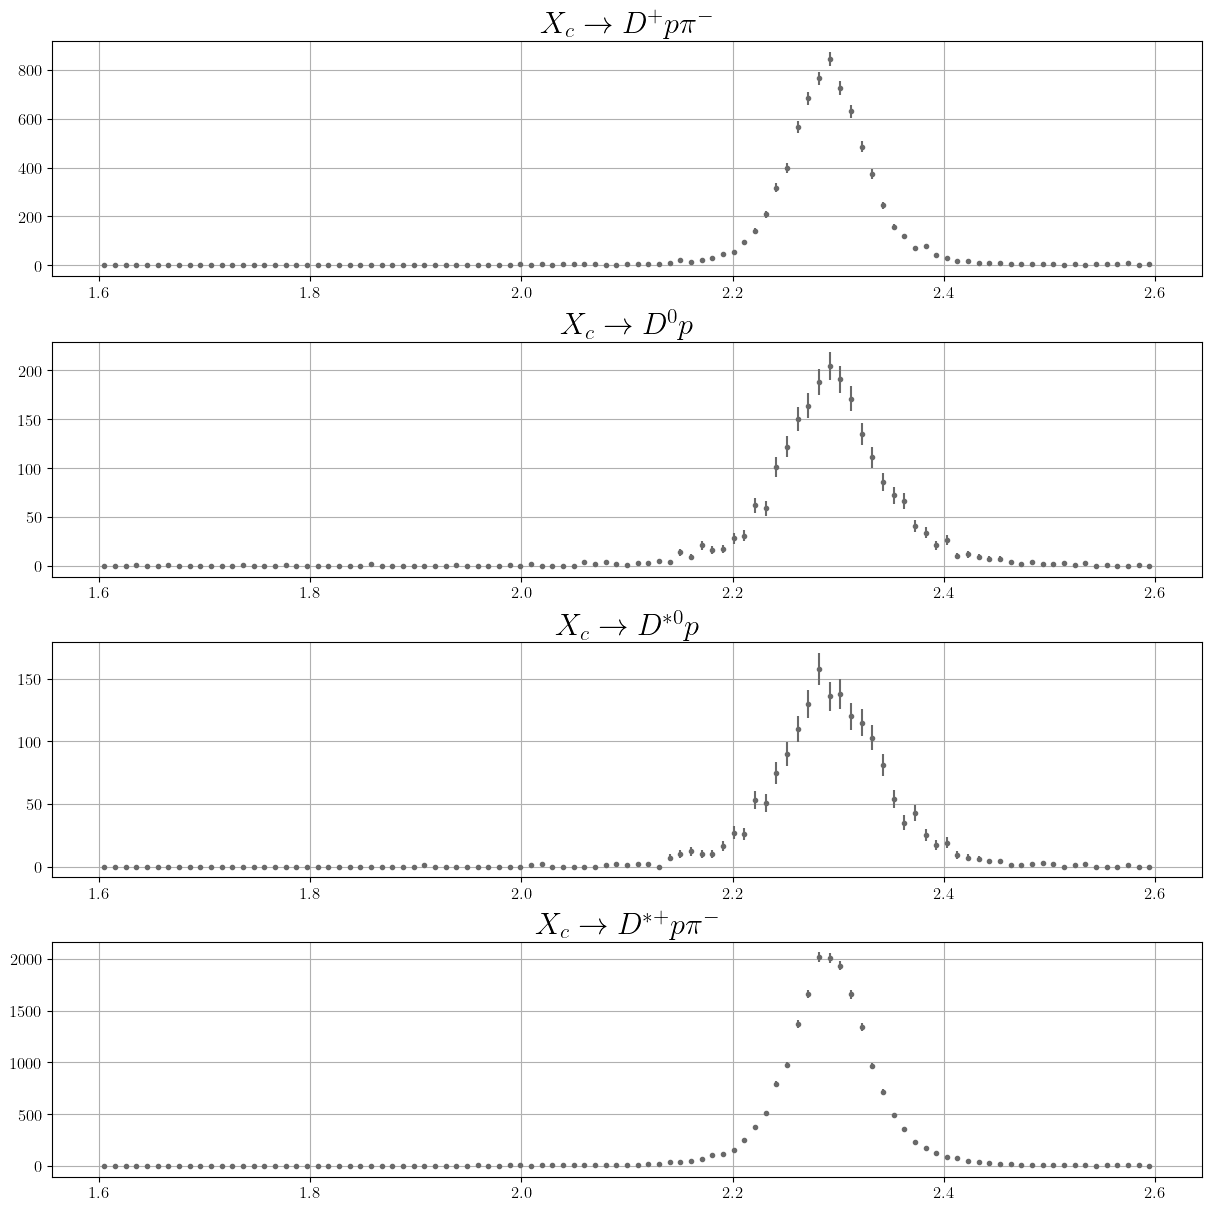
\includegraphics[width=1\linewidth]{img/MC_sig.png}
    \caption{Распределение сигнальных событий по каналам.}
    \label{MC_sig}
\end{figure}

Распределение аппроксимировалось функцией из трёх гауссианов для каналов с заряженными треками и из двух гауссианов для каналов с нейтральными треками с произвольной нормировкой (где $N$ — количество событий, вычисленное методом максимального правдоподобия, $N_r$ — истинное количество событий). Использование нескольких гауссианов обусловлено различием разрешения каналов $D$-мезонов:

\begin{equation}
    f_{\text{sig}} = C_{\text{sig}}\sum_{i=1}^{2,3} A_i N_i(x)
\end{equation}

где $\sum_i A_i = 1$ для сохранения нормировки. Итог аппроксимации (рис. \ref{MC_sig_fit}).

\begin{figure}[H]
    \centering
    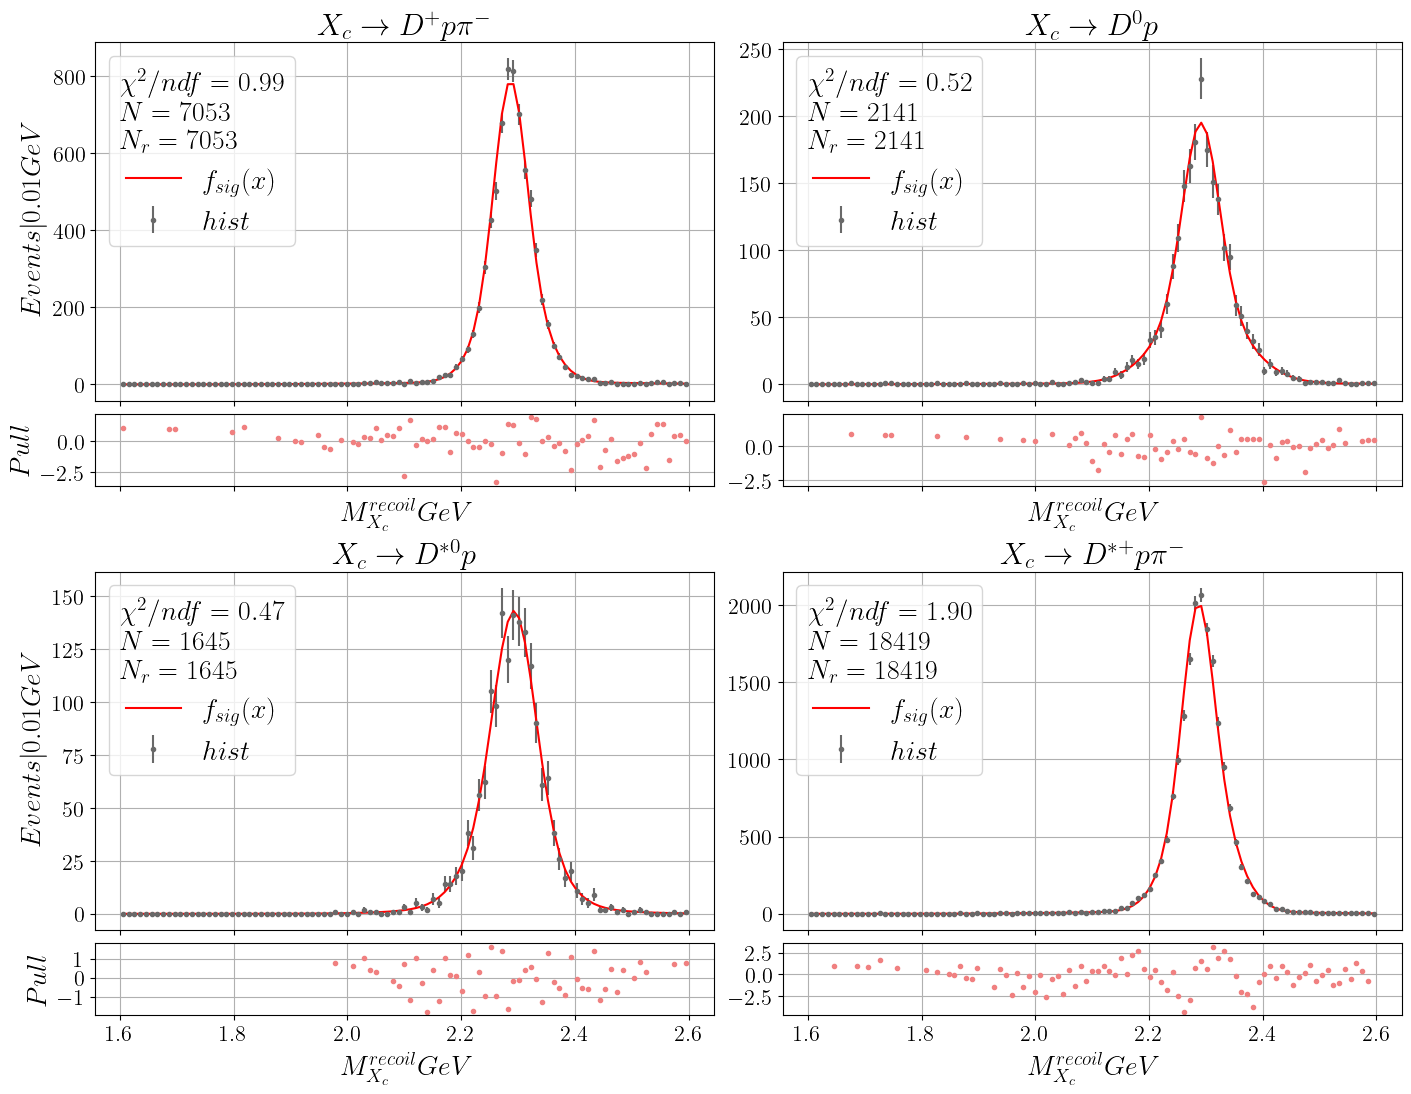
\includegraphics[width=1\linewidth]{img/MC_sig_fit.png}
    \caption{Распределение сигнальных событий по каналам.}
    \label{MC_sig_fit}
\end{figure}

Помимо сигнала рассматриваются два вида фоновых событий. Первый описывает потери в детекторе с критериями отбора:

\begin{itemize}
    \item Каждая детектируемая частица правильно идентифицирована, то есть треку была присвоена верная гипотеза на основе информации из Монте-Карло.
    \item $E_{\text{beam}} - E_{X_c} - E_{\Lambda_c} > 0.015$ ГэВ.
\end{itemize}

В итоге получено распределение (рис. \ref{MC_bg_lost}).

\begin{figure}[H]
    \centering
    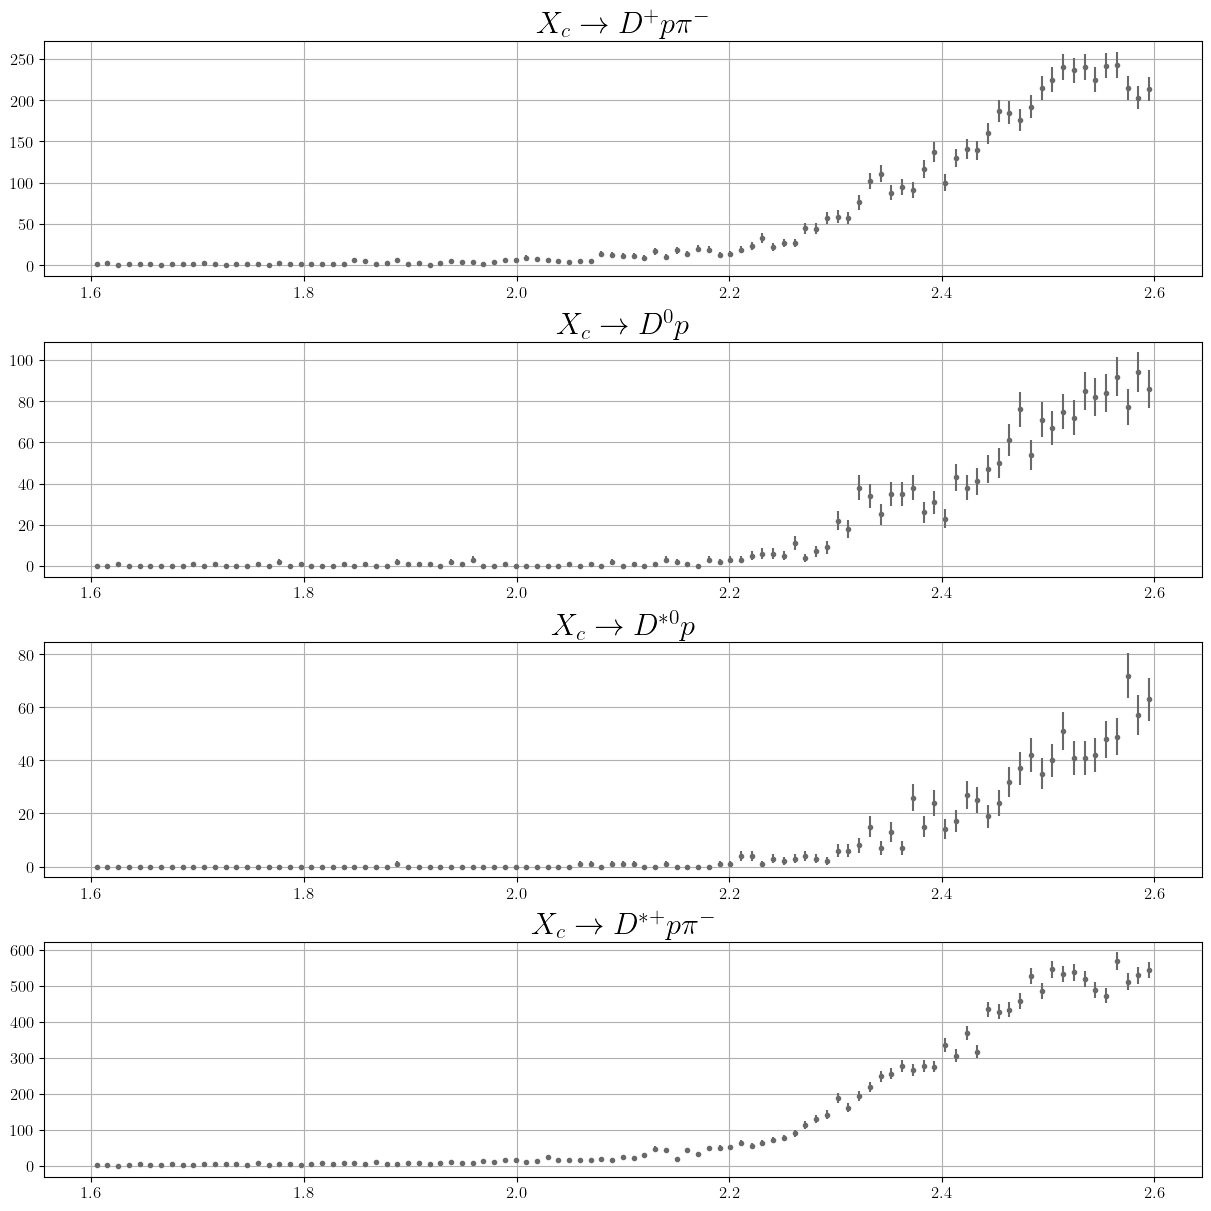
\includegraphics[width=1\linewidth]{img/MC_sqr_bg.png}
    \caption{Распределение событий с потерями.}
    \label{MC_bg_lost}
\end{figure}

Распределение показывает рост от $M_{\Lambda_c}$, так как если частица потеряна, то восстановленная масса должна быть:

\begin{equation}
    p_{X_c} + p_{\Lambda_c} + p_{\text{lost}} = p_{\text{beam}} \implies \abs{p_{\text{beam}} - p_{X_c}} = \abs{p_{\Lambda_c} + p_{\text{lost}}}
\end{equation}

Для описания распределения использовались два корня, начинающих рост от $M_{\Lambda_c}$ (потеря фотона) и $M_{\Lambda_c} + M_{\pi^0}$ (потеря $\pi^0$-мезона). Размытие распределений согласовано с размытием пика сигнала, и корни свёртываются с функцией распределения сигнала. В итоге распределение аппроксимировалось функцией:

\begin{equation}
    F_{\text{lost}} = C_{\text{lost}} \int f_{\text{sig}}(x)\cdot f_{\text{lost}}(x-s) dx
\end{equation}

где

\begin{equation}
    f_{\text{lost}}(x) = c_1\sqrt{\inner{x - M_{\pi}} \cdot \theta\inner{x - M_{\pi}}} + c_2\sqrt{x \cdot \theta\inner{x}}
\end{equation}

Результат подгонки (рис. \ref{MC_bg_lost_fit}).

\begin{figure}[H]
    \centering
    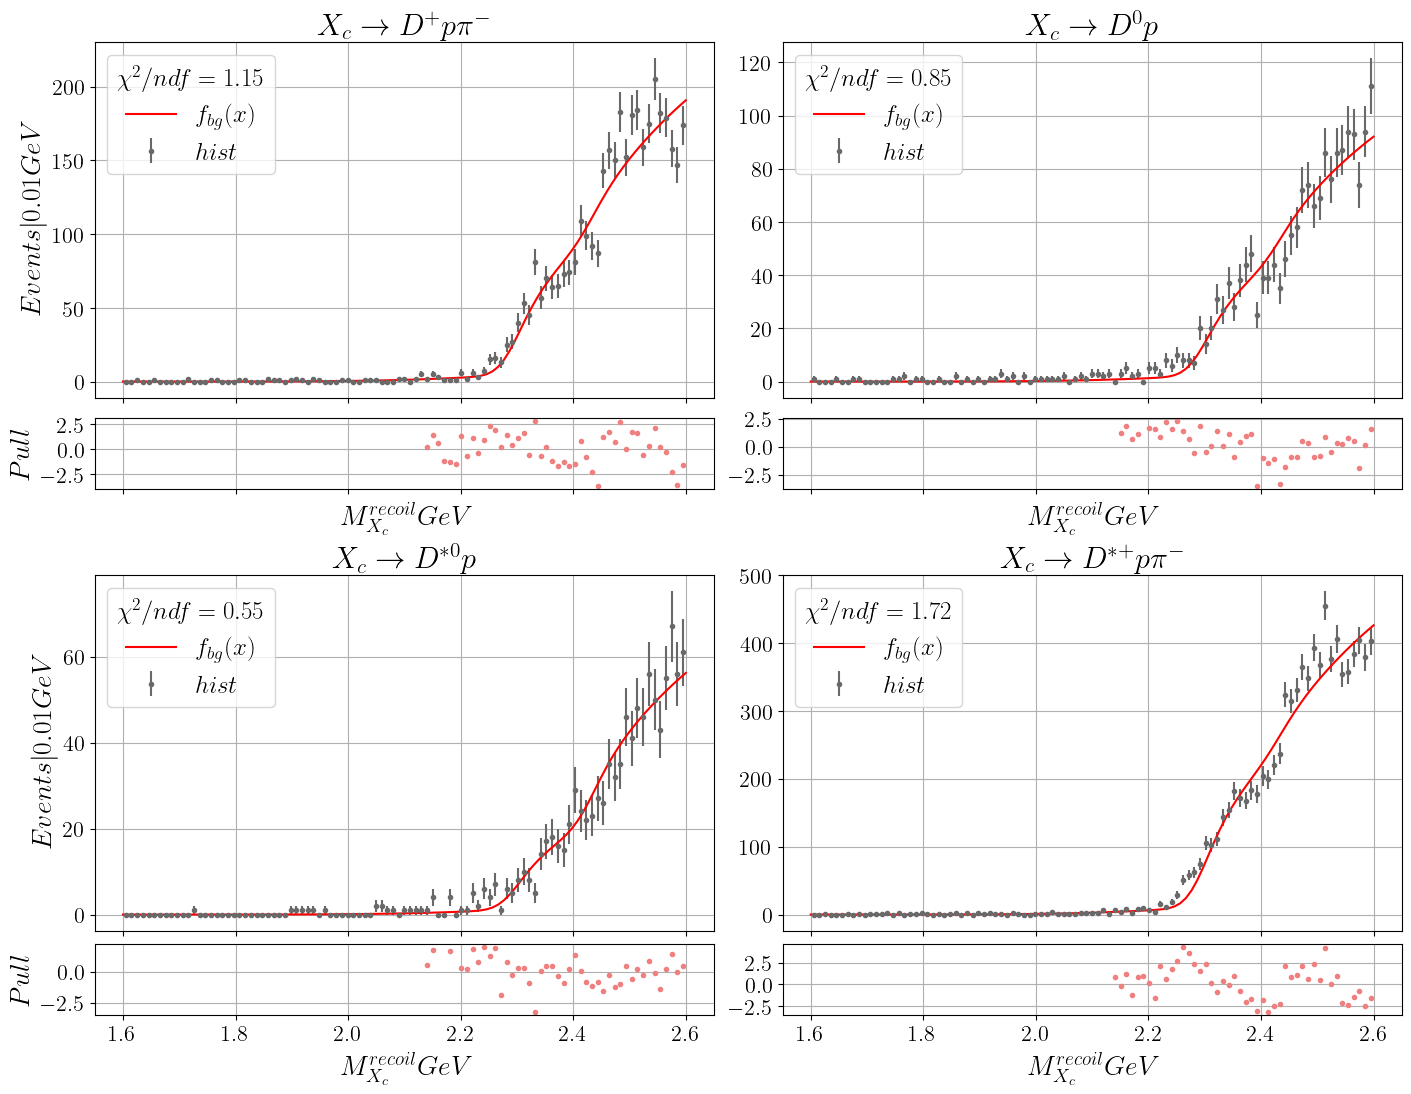
\includegraphics[width=1\linewidth]{img/MC_sqr_bg_fit.png}
    \caption{Распределение событий с потерями.}
    \label{MC_bg_lost_fit}
\end{figure}

Второй вид фона — комбинаторный, его распределение представлено на рис. \ref{MC_comb}.

\begin{figure}[H]
    \centering
    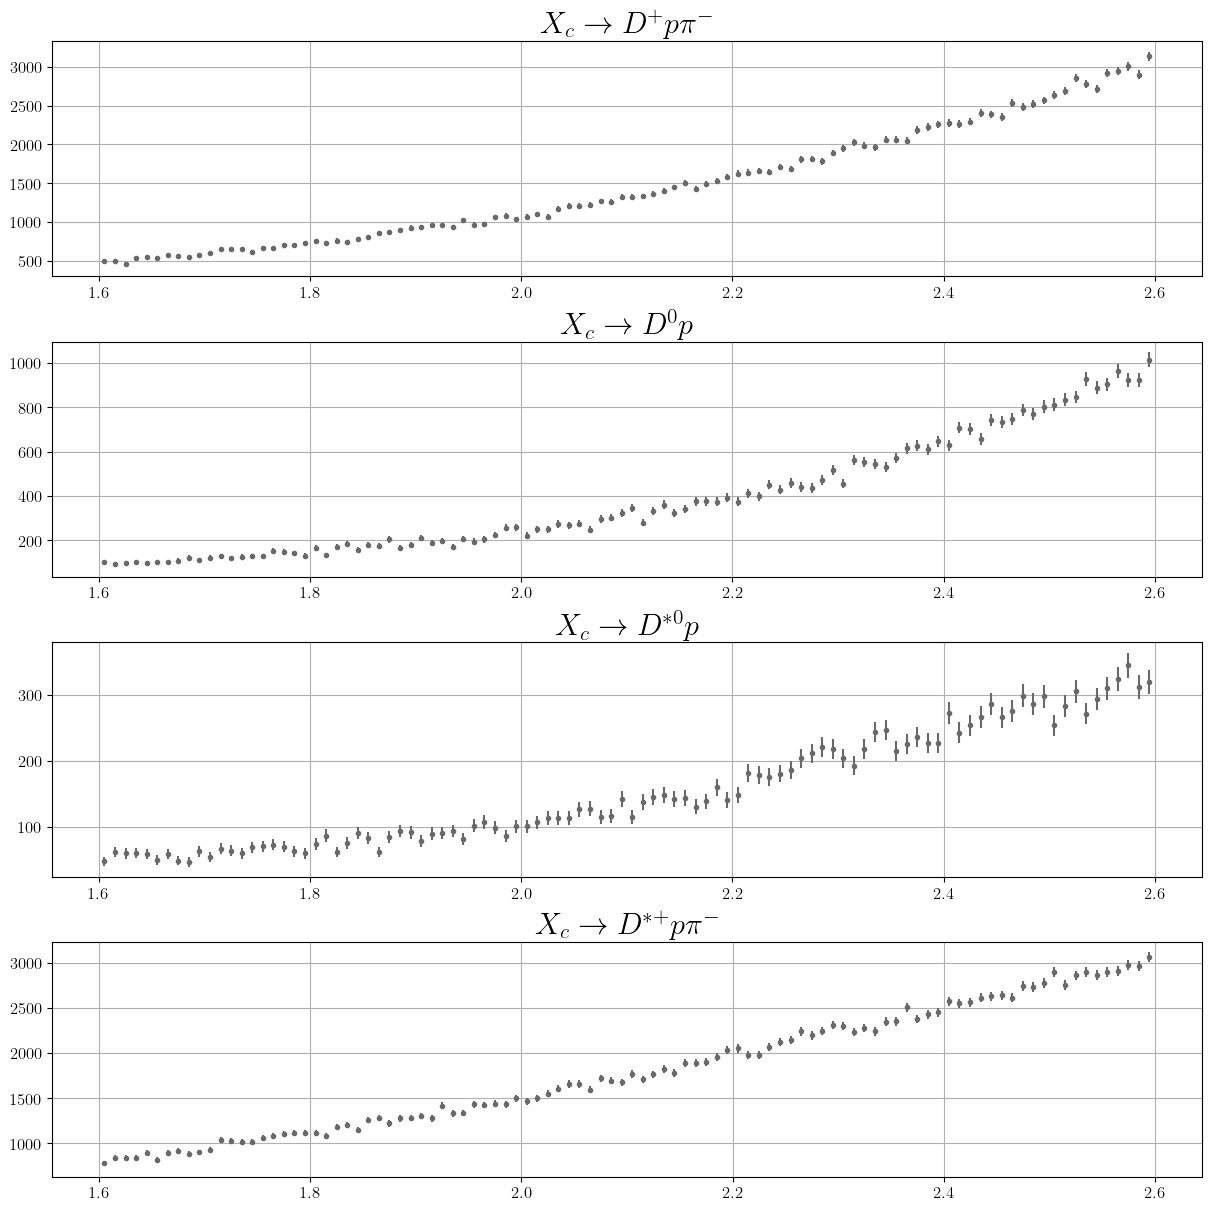
\includegraphics[width=1\linewidth]{img/MC_comb.png}
    \caption{Распределение событий комбинаторного фона.}
    \label{MC_comb}
\end{figure}

Комбинаторный фон стандартно описывается экспонентой, так как вероятность ошибочной идентификации частиц и формирования $X_c$ увеличивается с количеством частиц в событии. Для улучшения описания в распределение добавлен линейный полином.

Аппроксимация распределения выполнялась функцией:

\begin{equation}
    F_{\text{comb}} = \exp\insqr{\inner{x - \mu}\lambda} + c_0 + c_1 x
\end{equation}

Результат подгонки (рис. \ref{MC_comb_fit}).

\begin{figure}[H]
    \centering
    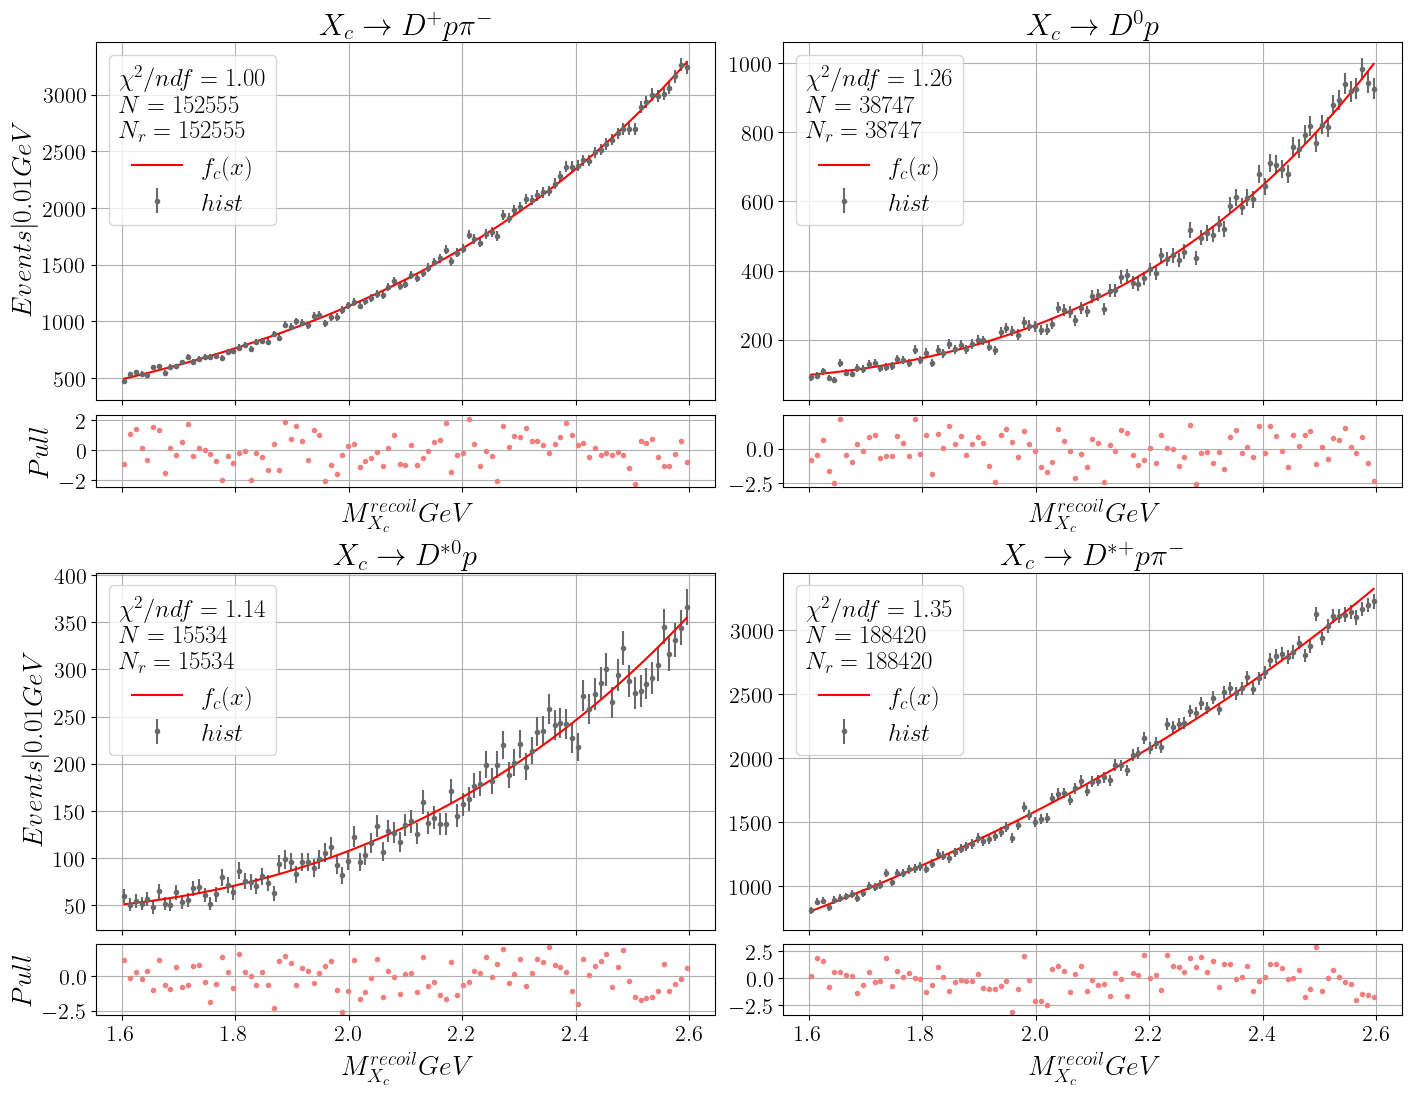
\includegraphics[width=1\linewidth]{img/MC_comb_fit.png}
    \caption{Распределение событий комбинаторного фона.}
    \label{MC_comb_fit}
\end{figure}


\section{Поиск $\Lambda_c$}

На основе выбранных нами каналов $X_c$ писанных в предыдущем разделе 
обираем события в котрых выполняется условие 

\begin{equation}
    \abs{p_{e^+} + p_{e^-} - p_{X_c}}^2 \leq 3 GeV
\end{equation}

Так как в идельных условиях эта влечина должна быть равна квадрату $M^{real}_{\Lambda_c} = 2226.46 MeV$, 
таким образом мы откинем множетво событий котрые затагировали 
возбужденные состояния $\Lambda_c$ или поряли трек.

В отобранных событиях мы будем собирать $\Lambda_c$ барионы. 
По каналам $\Lambda_c^+ \to \Lambda \pi^+; \Lambda \nu_e e^+; \Lambda \nu_\mu \mu^+$.



\newdot Для отбора $\Lambda \to p \pi$ требуем 

$$
\abs{ M_{\Lambda_c} - M^{real}_{\Lambda_c} } < 30 \text{ MeV}; 
\ \rho_{\Lambda_c} > 1 \text{ mm}; \ z_{\Lambda_c} > 1 \text{ cm}; 
\ \cos \theta_{\Lambda_c} > 0.99;
\ \mathfrak{L}_{p/K } > 0.6 
$$

\newdot Для отбора $e^\pm$ требем $p_{e^\pm} \geq 0.6 GeV$, чтобы долетел до SVD 
детектора где он в ходе $e^- \to \gamma e^- \to 2e^- e^+$ распадается электронн-фотонным ливнем, 
что позволяет его олично индетефицировать, поэтому критерий на $L(e) > 0.1$ не такой строгий.

\newdot Аналогично отбора $\mu^\pm$ требем $p_{\mu^\pm} \geq 0.6 GeV$, чтобы долетел до KLM, 
где идентификация мюнов еще лучше поэтому требуем $L(\mu) > 0.01$ 


\newdot Комбинируем $\Lambda_c$ с массовым окном $50 MeV$.

\newdot Независимо от работы \cite{BelleDetector2002}, среди моножетва $\infig{d_n}$, 
идентифицированных как кандидаты на дочерние продукты распада $\xi$ частици, 
можно использовать знание о том, что импульсы продуктов распада должны исходить 
из вершины распада. Это позволяет откорректировать измеренные импульсы с учётом 
погрешностей, чтобы они соответствовали данной гипотезе (в дальнейшем это будет 
называться "фит в вершину"). Аналогично, на основании инвариантной массы, 
известной для $\xi$, можно корректировать величины импульсов дочерних частиц 
так, чтобы $M_{p} = \sqrt{\sum_n \inner{p_n}_\gamma \inner{p_n}^\gamma}$ 
совпадала с $M^{real}_{\xi}$, где $p_n$ --- 4-импульс сответствующий $d_n$ 
из $\infig{d_n}$. Этот метод будет называться "фит в массу". Были использованы 
алгоритмы для фита в вершину и в массу принятые в коллаборации KEK, и описанные 
в \cite{Krohn2021}.

По итогу делаем фиты в вершину, а после в массу для всех собранных частиц это 
$\Lambda_c, D^{\pm}, D^0, D*^{\pm}, D*^0, \Lambda, K_s^0$.

\newdot Для импульс $X_c$ фитируем так чтобы $\abs{p_{e^+} + p_{e^-} - p_{X_c}}^2 = M^2_{\Lambda_c}$, 
подробно алгоритм описан в Appendix \ref{fit_rec_mass}. 

 









\section{Анализ Monte Carlo}

\subsection*{Генерация и отбор событий.}

Для отбора наилучших кандидатов было предложено использовать события, сгенерированные с помощью MC для распада $e^+e^- \to c\bar{c}$. На основе полученной статистики предлагается обучить модель Random Forest для отбора истинных событий на тагирующей стороне. Поскольку основной целью данной работы является измерение формфактора $\Lambda_c$, модель не будет использоваться для идентификации кандидатов на $\Lambda_c$ в исследуемой стороне.

Применяя аналогичные критерии отбора к тагирующей стороне, был добавлен канал $\Lambda_c^{\text{tag}} \to p K \pi$, что позволило увеличить статистическую значимость, исключив при этом канал $\Lambda_c \to \Lambda \ell \nu_\ell$ из анализа тагирующей стороны. В результате этого отбора удалось выделить следующее количество событий.

\begin{figure}[H]
    \centering
    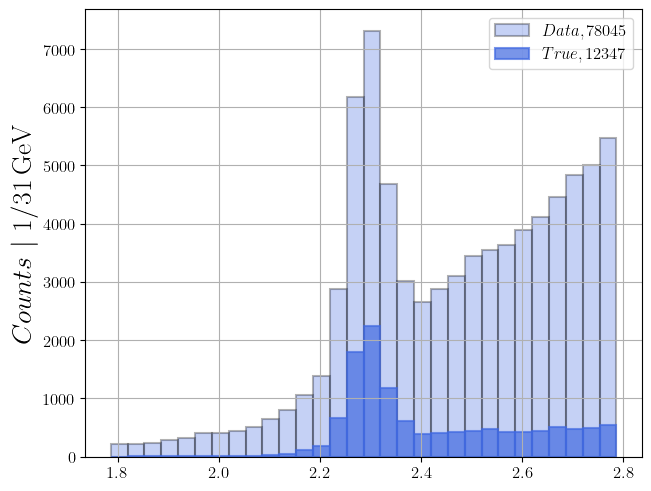
\includegraphics[width=0.7\linewidth]{img/mc_tr.png}
    \caption{Сгенерированные и истинные события в MC, распределение по восстановленной массе $\Lambda_c$.}
\end{figure}


\subsection{Отбор истинных кандидатов в событиях Monte Carlo}


В качестве признаков использовались: $M^{rec}_{\Lambda_c}, \abs{p_{ach}}, M_{ach}, \abs{p_{\pi}}, M_{\pi}, \abs{p_{X_c}}, \abs{p_{X_c}}, M_{X_c}, E_{cm}, \abs{p_{cm}}$, и углы между всеми импульсами в системе центра масс и главное предполагаемый канал распада $X_c$, были введены следующие обозначения $ach$ --- носистель $\bar c$,  $cm$ --- система центра масс. Целевая метка определялась из информации присвоенным MC генератором.

Для обучения был использован Random Forest классификатор с количеством деревьев 4000, глубиной деревьев до 200 и настройкой параметров для борьбы с несбалансированностью классов. Модель обучалась на 60\% данных, оставшиеся 40\% использовались для тестировани.

Поскольку в одном событии может быть несколько комбинаций, на каждом шаге выполнялась фильтрация кандидатов. Сначала отбирались события с вероятностью больше порога $L = 0.4$, а затем среди всех кандидатов в одном событии выбирался лучший на основе максимальной вероятност

Для оценки производительности модели был построен ROC-кривая (рис. \ref{ROC}) и рассчитана площадь под кривой (AUC). Кроме того, предсказанные вероятности были использованы для выбора порога вероятности, выше которого событие классифицируется как содержащее истинного кандидат

Были построены гистограммы (рис. \ref{hist}) для сравнения истинных и предсказанных кандидатов, а также для анализа ошибок классификации (FP, FN, TP, TN). Это позволило оценить распределение признаков для разных категорий событий и уточнить работу классификатора на тестовой выборке.

\begin{figure}[H]
    \centering
    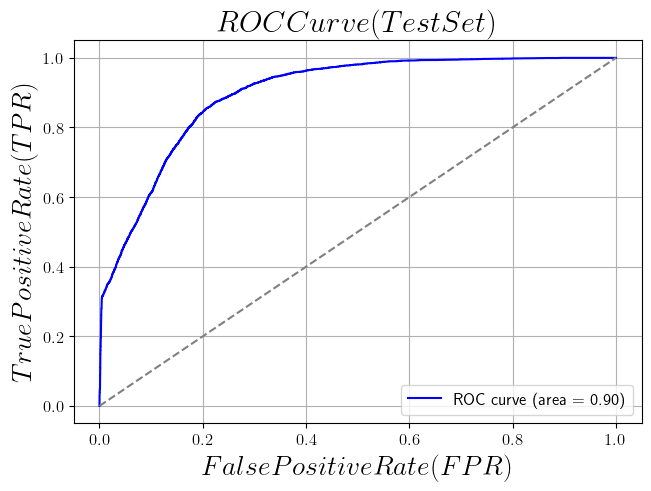
\includegraphics[width=0.7\linewidth]{img/ROC_f.png}
    \caption{ROC кривая классификатора.}
    \label{ROC}
\end{figure}

\begin{figure}[H]
    \centering
    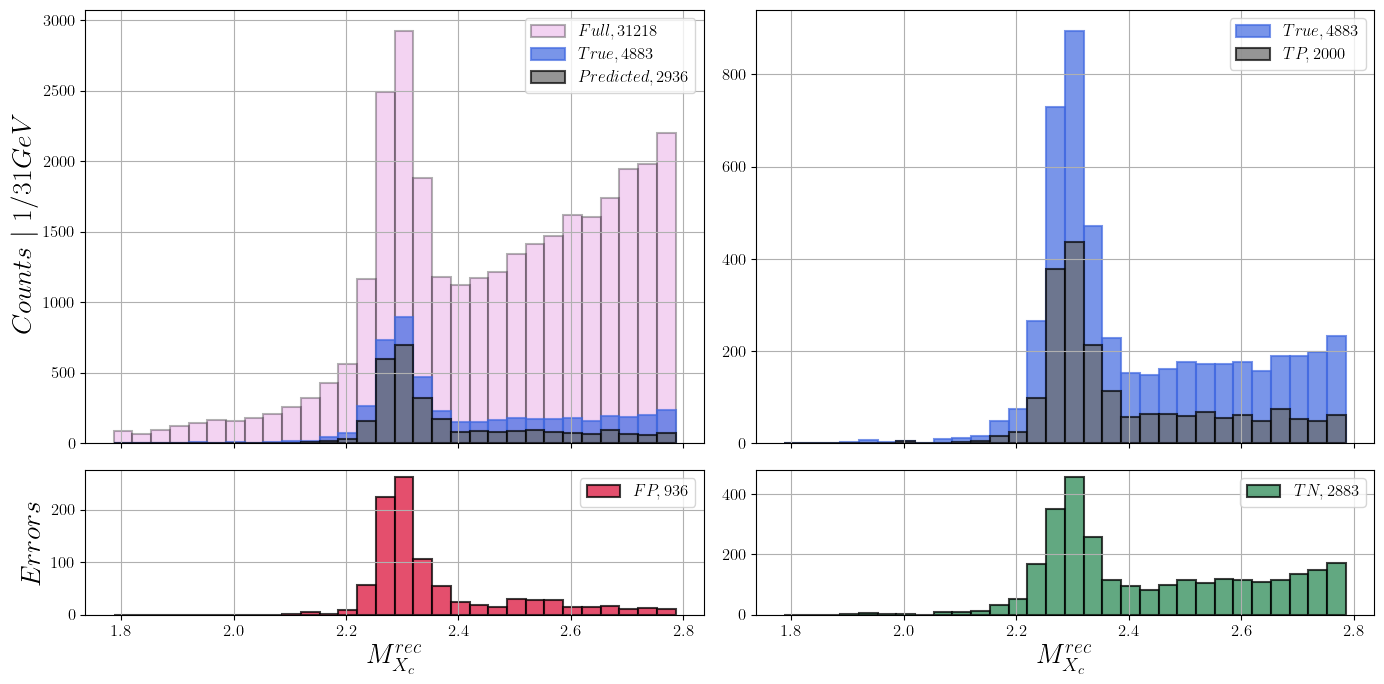
\includegraphics[width=1\linewidth]{img/MC_res.png}
    \caption{Результаты классификатора на тестовой выборке.}
    \label{hist}
\end{figure}

Таким образом данные полученные в разделе \ref{Lamc:search} так же проходят через данный классификатор.

На данный момент классификатор и дальныешие аппроксимации все еще улучшаются, 
поэтому результаты не являются оканчательными.


\section{Измерение продольной поляризации $\Lambda_c \to \Lambda \pi$}

С помощью формализма спиральных амплитуд \textbf{\cite{Richman}} можно описать процесс 
$\Lambda_c \to \Lambda \pi$ и получить его угловое распределение с 
учётом продольной поляризации. На рис. \ref{def:val} показаны определения 
наблюдаемых величин. 

\begin{figure}[H]
    \centering
    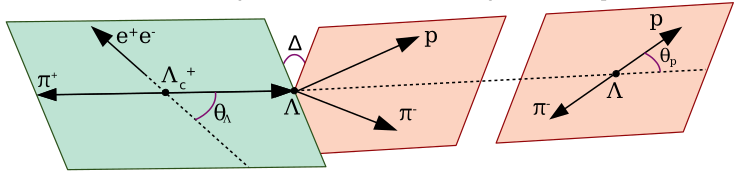
\includegraphics[width=0.7\linewidth]{img/lpi_def.png}
    \caption{Определение переменных.}
    \label{def:val}
\end{figure}

Амплитуда записывается следующим образом:

\begin{equation}
    A_{\llp{c} \llp{p}} = \sum_{\llp{c}} A_{\llp{c}} D^{1/2\dag}_{\llp{c} \llp{p}}\left(\phi_\lambda, \theta_\Lambda, -\phi_\Lambda \right) D^{1/2\dag}_{\llp{c} \llp{p}} B_{\llp{p}} D^{1/2}_{\llp{c} \llp{p}}\left(\phi_\lambda, \theta_\Lambda, -\phi_\Lambda \right)
\end{equation}

Где $\llp{p}$ --- спиральность протона, 
$A_{\llp{c}}$ --- спиральная амплитуда $\Lambda_c \to \Lambda \pi^+$, 
$B_{\llp{c}}$ --- спиральная амплитуда $\Lambda_c \to \Lambda \pi^-$,





\section{Измерение формфактора полулептонных распадов $\Lambda_c$}

\subsection{Теория}

Процедура измерения формфакторов в распадах $\Lambda_c \to \Lambda l \nu_l$
уловому распредлению. Переменные углового распределения представлены 
на (рис. \ref{lc_l_l_nu:def}). 

\begin{figure}[H]
    \centering
    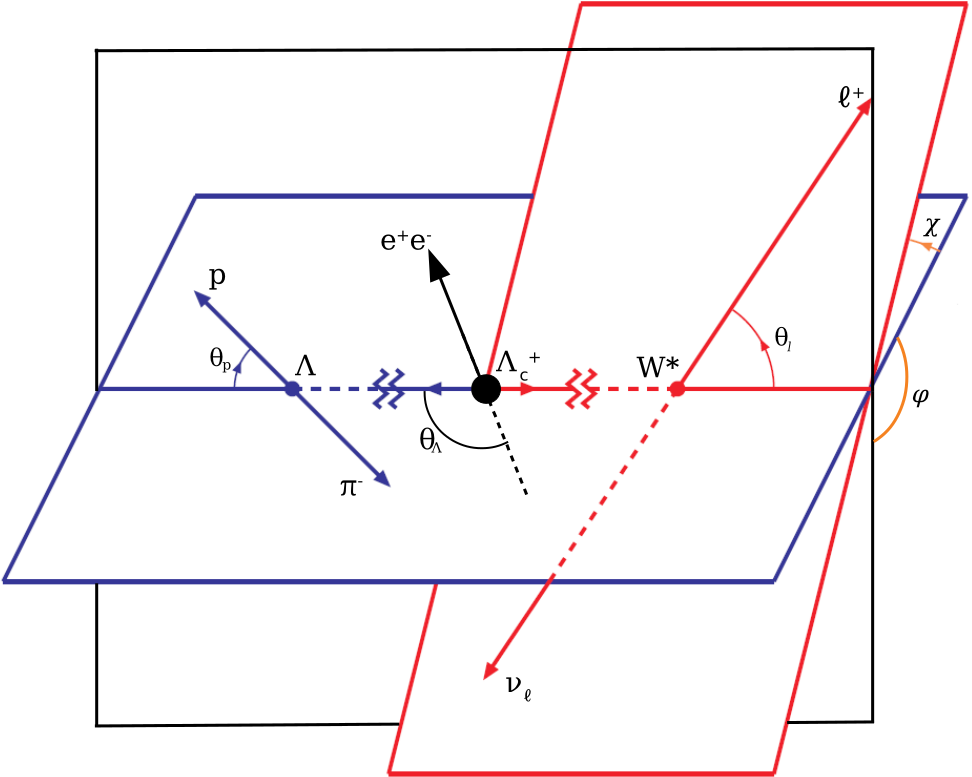
\includegraphics[width=0.7\linewidth]{img/lc_l_l_nu_def.png}
    \caption{Определение переменных углового распределения в распадах  $\Lambda_c \to \Lambda l \nu_l$.}
    \label{lc_l_l_nu:def}
\end{figure}

Амплитуда распадов 
$\Lambda_c \to \Lambda W^*, W^* \to l^+ \nu_l, \Lambda \to p \pi$:


\begin{equation}
    M_{\lambda_{\Lambda_c}\lambda_{p}\lambda_{l}\lambda_{\nu}} 
    = 
    \sum_{\lambda_{\Lambda},J,\lambda_{W}} H_{\lambda_{\Lambda},\lambda_{W}} D^{\frac{1}{2} \dagger}_{\lambda_{\Lambda_c},\lambda_{\Lambda}-\lambda_{W}}(\phi_{\Lambda}, \theta_{\Lambda}, -\phi_{\Lambda}) B_{\lambda_{p}} D^{\frac{1}{2} \dagger}_{\lambda_{\Lambda},\lambda_{p}}(\phi_{p}, \theta_{p}, -\phi_{p}) h_{\lambda_{l},\lambda_{\nu}} D^{J \dagger}_{\lambda_{W},\lambda_{l}-\lambda_{\nu}}(\phi_{l}, \theta_{l}, -\phi_{l}),
\end{equation}


где $\theta_l, \phi_l$ --- полярный и азимутальный углы импульса лептона 
в системе отсчёта  $W^*$-бозона, имеющую ось $z$, которая направлена 
противоположно импульсу $\Lambda^+_c $-бариона, 
$\lambda_l$ --- спиральность лептона, 
$\lambda_\nu$ --- спиральность нейтрино, 
которая принимает значения $-\frac{1}{2}$ у $\nu_l$, $\frac{1}{2}$ у $\bar \nu_l$, 
то есть зависит от знака заряда. 
Для вычисления спиральной амплитуды $h_{\lambda_l, \lambda_\nu}$, 
в системе покоя $W^*$-бозона, ось $z$ направлена вдоль импульса лептона 
$\vec{p}_l$ и использовались выражения биспиноров:

\begin{equation}
    \bar{u}_l\inner{\pm \frac{1}{2}} = \sqrt{E_l + m_l} \inner{\chi^{\dagger}_{\pm}, \frac{\mp |\vec{p}_l|}{E_l + m_l} \chi^{\dagger}_{\pm}}, 
    \quad 
    \bar{u}_l\inner{-\frac{1}{2}} = \sqrt{E_\nu} \inner{\chi^{\dagger}_{-}, \chi^{\dagger}_{-}},
\end{equation}
\begin{equation}
    v_l\inner{\pm \frac{1}{2}} = \sqrt{E_l + m_l} \inner{ \frac{\mp \abs{\vec{p}_l}}{E_l + m_l} \chi_{\pm}, \chi_{\pm} },
    \quad
    v_\nu\inner{+\frac{1}{2}} = \sqrt{E_\nu} \inner{-\chi_-, -\chi_-},
\end{equation}
\begin{equation}
    v_\nu\inner{+\frac{1}{2}} = \sqrt{E_\nu} \inner{-\chi_-, -\chi_-},
\end{equation}

4-векторы поляризации виртуального $W$-бозона: $\epsilon^\mu(t) = (1; 0, 0, 0), \epsilon^\mu(0) = (0; 0, 0, 1), \epsilon^\mu(\pm 1) = \frac{1}{\sqrt{2}} (0; \mp 1, -i, 0)$. 
Вследствие сохранения полного момента импульса $\lambda_W = \lambda_l - \lambda_\nu$ и вида слабого тока из СМ:

\begin{equation}
    h_{\lambda_l = \frac{1}{2}, \lambda_\nu = \frac{1}{2}} = \bar{u}_l\inner{-\frac{1}{2}} \gamma^\mu (1 + \gamma_5) v_\nu \inner{+\frac{1}{2}}
    \begin{cases}
    \epsilon_\mu(-1) \\
    \epsilon_\mu(t), \epsilon_\mu(0)
    \end{cases},
\end{equation}
\begin{equation}
    h_{\lambda_l = \pm \frac{1}{2}, \lambda_\nu = - \frac{1}{2}} = \bar{u}_l \inner{- \frac{1}{2}} \gamma^\mu (1 + \gamma_5) v_l \inner{\pm \frac{1}{2}}
    \begin{cases}
    \epsilon_\mu(1) \\
    \epsilon_\mu(t), \epsilon_\mu(0)
    \end{cases}.
\end{equation}

cпиральные амплитуды $h_{\lambda_l,\lambda_\nu}$ подразделяются на два случая, связанные
с произошедшим или не произошедшим переворотом спина лептона, то
есть изменением его спиральности на противоположную после распада $W^*$-бозона:

\begin{eqnarray}
    \text{без переворота спина} \inner{\lambda_W = \mp 1}: \ \abs{h_{\lambda_l = \mp 1/2, \lambda_\nu = \pm 1/2}}^2 = 8 \inner{q^2 - m_l^2}\\
    \text{перворотом спина} \inner{\lambda_W = t, 0}: \ \abs{h_{\lambda_l = \pm 1/2, \lambda_\nu = \pm 1/2}}^2 = 8 \cfrac{m_l^2}{2q^2}\inner{q^2 - m_l^2}
\end{eqnarray}

Так как порядка сотни восстановленных сигнальных событий 
недостаточно для измерения всех шести формфакторов в общем случае, 
были сделаны предположения:

\newdot $m_l = 0$;

\newdot $H_{\lambda_\Lambda \lambda_W} \in \re$;

\newdot Распад $\Lambda_c \to \Lambda l \nu_l$ происходит согласно теории тяжелых квакров тоесть $c \to s W^*$;

\newdot Вид формфакторов соответствует модели $KK$ согласованой с торией тяжелых кварков.

Предоложения, писанные выше были также сделаны в работе \cite{CLEO2023}, но в отличие от них 
в данной работе не делается предположения о равномерном распределении направления спина $\Lambda$,
а распределен согласно измерениям продленным в разделе \ref{helisity:Lambda}.

Проделывая вычиления аналогичные \ref{helisity:amplitud:Lam}-\ref{spin:Lam:pdf} получим из:

\begin{eqnarray}
    \frac{d\Gamma}{dq^2 d\cos\theta_\ell d\cos\theta_p d\cos\theta_d d\phi_\ell d\phi_p d\chi} = 
    p\sum_{\lambda_W \lambda_l \lambda_\nu } \abs{M_{\lambda_{\Lambda_c}\lambda_{p}\lambda_{l}\lambda_{\nu}} }^2
\end{eqnarray}

\begin{eqnarray}
    d\Gamma = \cfrac{1+P_L}{2}d\Gamma_{+1/2} + \cfrac{1-P_L}{2}d\Gamma_{-1/2}
\end{eqnarray}

Упрощённая форма углового распределения:

\begin{multline}
    \frac{d\Gamma}{dq^2 d\cos\theta_\ell d\cos\theta_p d\cos\theta_d d\phi_\ell d\phi_p d\chi} \propto q^2 \sqrt{Q_+ Q_-} f^{\Lambda_\ell \nu_\ell}_{\text{sig}} \times \\
    \left\{ H_{1\frac{1}{2}}^2 \inrad{1 - P_L \cos\theta_\Lambda} \inrad{1 + \alpha_\Lambda \cos\theta_p} \inrad{1 \pm \cos\theta_\ell}^2 + \right. \\
    + H_{-1\frac{1}{2}}^2 \inrad{1 + P_L \cos\theta_\Lambda} \inrad{1 - \alpha_\Lambda \cos\theta_p} \inrad{1 \mp \cos\theta_\ell}^2 +\\
    + 2 \sin^2\theta_\ell \left[ H_{0\frac{1}{2}}^2 \inrad{1 + P_L \cos\theta_\Lambda} \inrad{1 + \alpha_\Lambda \cos\theta_p} + H_{0\frac{1}{2}}^2 \inrad{1 - P_L \cos\theta_\Lambda} \inrad{1 - \alpha_\Lambda \cos\theta_p} \right] - \\
    - 2\sqrt{2} \alpha_\Lambda \sin\theta_p \sin\theta_\ell \cos\chi \left[ H_{1\frac{1}{2}} H_{0\frac{1}{2}} \inrad{1 - P_L \cos\theta_\Lambda} \inrad{1 \mp \cos\theta_\ell} + H_{-1\frac{1}{2}} H_{0\frac{1}{2}} \inrad{1 + P_L \cos\theta_\Lambda} \inrad{1 \pm \cos\theta_\ell} \right] -\\
    - 2\alpha_\Lambda P_L \sin\theta_\Lambda \sin\theta_p \sin^2\theta_\ell \left[ 2H_{0\frac{1}{2}} H_{0\frac{1}{2}} \cos\varphi + H_{1\frac{1}{2}} H_{-1\frac{1}{2}} \cos(\varphi + 2\chi) \right] +\\
    + 2\sqrt{2} P_L \sin\theta_\Lambda \sin\theta_\ell \cos(\varphi + \chi) \left[ H_{1\frac{1}{2}} H_{0\frac{1}{2}} \inrad{1 + \alpha_\Lambda \cos\theta_p} \inrad{1 \pm \cos\theta_\ell} \right] \\
    \left.+ H_{-1\frac{1}{2}} H_{0\frac{1}{2}} \inrad{1 - \alpha_\Lambda \cos\theta_p} \inrad{1 \mp \cos\theta_\ell} \right\}
\end{multline}

\subsection{Измерения продольной поляризации}

В итоге сигнальная фанкция:

\begin{equation}
    f_{S}^{\Lambda l \nu} (\mathbf{y}, \xi; R, M_{\text{pole}}) = \frac{\varepsilon_{\Lambda l \nu} (\mathbf{y}, \xi) f_{\text{sig}}^{\Lambda l \nu} (\mathbf{y}; R, M_{\text{pole}})}{\int \varepsilon_{\Lambda l \nu} (\mathbf{y}, \xi) f_{\text{sig}}^{\Lambda l \nu} (\mathbf{y}; R, M_{\text{pole}}) d\mathbf{y} d\xi},
\end{equation}

где $ R, M_{\text{pole}} $ --- параметры из модели $КК$, характеризующие форму 
и отношение двух независимых формфакторов, 
$\mathbf{y} = (q^2, \cos\theta_\Lambda, \cos\theta_p, \cos\theta_l, \varphi, \chi)$ 
--- переменные, от которых зависит $ f_{\text{sig}}^{\Lambda l \nu} $, 
$ \xi = (|p_{\Lambda_c}^{\text{CM}}|, \cos\theta_{\Lambda_c}^{\text{CM}}) $ --- 
переменные, не входящие явным образом в $ f_{\text{sig}}^{\Lambda l \nu} $, 
но влияющие на эффективность реконструкции событий; 
$\varepsilon_{\Lambda l \nu} $ --- полная эффективность восстановления, 
которая была получена следующим образом: для каждого бина двумерной гистограммы 
эффективности реконструкции (рис. \ref{l_l_nu:rec}) с сигнальными событиями 
создавалась многомерная гистограмма, разбитая на 
$ 5 \times 2 \times 2 \times 2 \times 3 \times 3 $ бина по переменным 
$ \mathbf{y} $, в каждом бине которой вычислялось отношение количества восстановленных событий к количеству 
сгенерированных. Многомерный интеграл в знаменателе $ f_S^{\Lambda l \nu} $ вычислялся численно.

\begin{figure}[H]
    \centering
    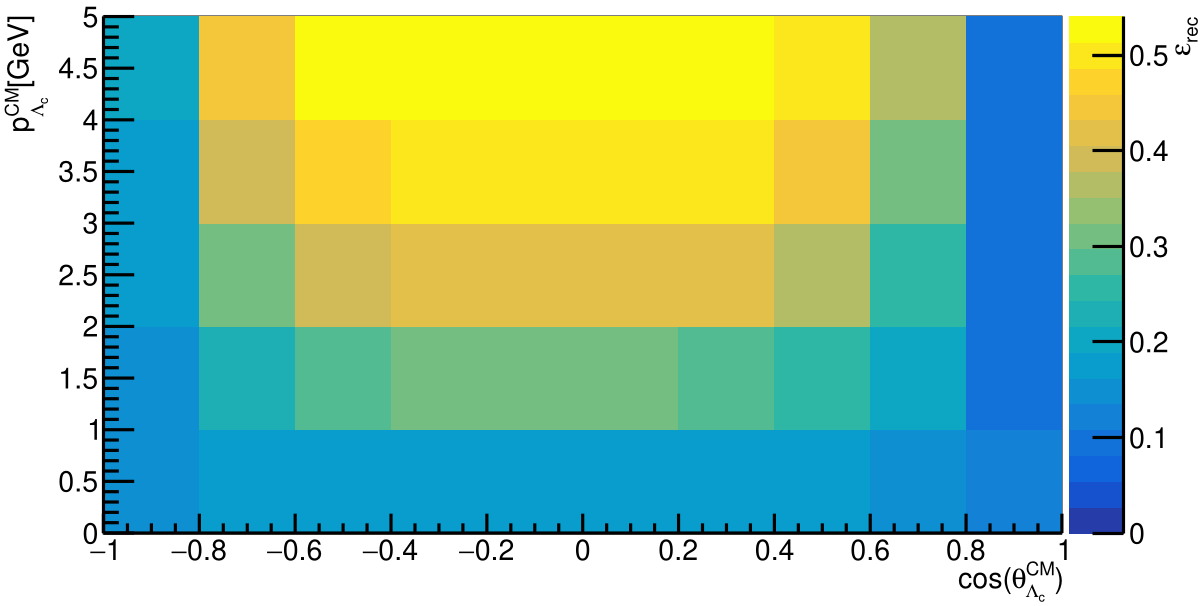
\includegraphics[width=1\linewidth]{img/l_l_nu_rec.png}
    \caption{Эффективность реконструкции распадов $\Lambda_c \to \Lambda e \nu_e$ в зависимости от
    косинуса полярного угла и величины импульса $\Lambda_c$-бариона в системе центра масс.}
    \label{l_l_nu:rec}
\end{figure}


Результы подгонки параметров методом максимального прадоподобия изображены на рис. \ref{l_l_nu:fit}


\begin{figure}[H]
    \centering
    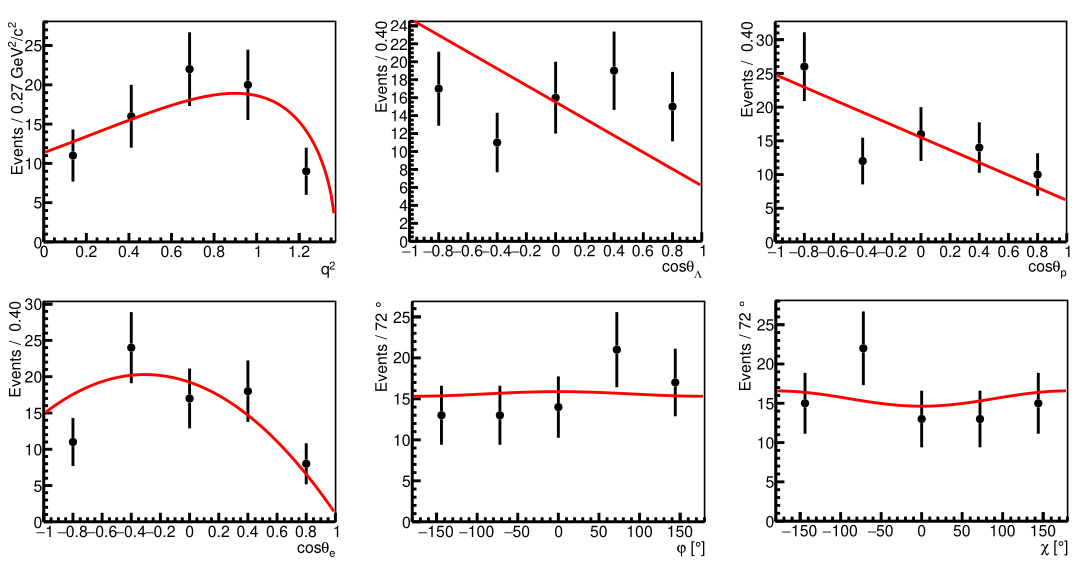
\includegraphics[width=1\linewidth]{img/l_l_nu_fit.png}
    \caption{Одномерные распределения событий $\Lambda_c \to \Lambda e \nu_e$ с наложенной
    функцией $f_{sig}$ с полученными параметрами}
    \label{l_l_nu:fit}
\end{figure}

\begin{eqnarray}
    \Lambda_c \to \Lambda e \nu_e: \ R = -0.52 \pm 0.13,\ M_{pole} = 1.82 ± 0.19 GeV
\end{eqnarray}





\mysection{Метод вычисления формфактора}

$\Lambda_c$ барион состит из $ucd$ кварков, в ходе распараспада 
$\Lambda_c \rightarrow \Lambda l \nu_l$ проискходит переход $c\to s$ 
посредством испускания $W^+$ бозона тоесть правиьно будет записвть $c\to s W^+$,
$W^+$ распадается на $W^+ \to l^+ \nu_l$, в итоге оставшиеся кварки 
$uds$ формируются в $\Lambda$ барион. Таким образом получим следующую 
феймановскую диаграмму.

\begin{figure}[H]
    \centering
    \begin{tikzpicture}
        \begin{feynhand}
            \vertex [particle] (i1) at (-3,4) {$u$};
            \vertex [particle] (i2) at (-3,3.5) {$d$};
            \vertex [particle] (i3) at (-3,3) {$c$};
            \vertex [particle] (f1) at (3,4) {$u$};
            \vertex [particle] (f2) at (3,3.5) {$d$};
            \vertex [particle] (f3) at (3,3) {$s$};
            \vertex (w1) at (0,3);
            \vertex (w2) at (0,2.5);
            \vertex (w3) at (0,2);
            \vertex (w4) at (1.5,1);
            \vertex [particle] (e) at (3,1.5) {$l^{-}$};
            \vertex [particle] (an) at (3,0.5) {$\bar{\nu}_{l}$};
            \propag [fermion] (i1) to (w1);
            \propag [fermion] (i2) to (w2);
            \propag [fermion] (i3) to (w3);
            \propag [fermion] (w1) to (f1);
            \propag [fermion] (w2) to (f2);
            \propag [fermion] (w3) to (f3);
            \propag [charged boson] (w3) to [edge label=$W^{-}$] (w4);
            \propag [fermion] (w4) to (e);
            \propag [anti fermion] (w4) to (an);        
        \end{feynhand}
    \end{tikzpicture}
\end{figure}

Переход $\Lambda_c \to \Lambda$ индуцирется слабым током $j_\mu$, 
котрый можно разложить по аксиальной и векторной части: 
$j_\mu = j_\mu^A + j_\mu^V$.
Обозначим волновые функции частиц
$B_{\Lambda_c} \inner{p_{\Lambda_c}, M_{\Lambda_c}} 
\to B_{\Lambda} \inner{p_{\Lambda}, M_{\Lambda}} 
+ l\inner{p_l, m_l} + \nu_l \inner{p_\nu, m = 0}$. 
Форм факторы выражаются как:
\begin{equation}
    \bra{B_{\Lambda_c} \inner{p_{\Lambda_c}, M_{\Lambda_c}}}
    j_\nu^V
    \ket{B_{\Lambda} \inner{p_{\Lambda}, M_{\Lambda}}} = 
    u_2^\dag \inner{\mathfrak F^V_1 \inner{q^2} \gamma_\nu + 
    \cfrac{\mathfrak F^V_2}{M_{\Lambda_c}} \inner{q^2} \sigma_{\mu\nu} q^\nu + 
    \cfrac{\mathfrak F^V_3}{M_{\Lambda_c}} \inner{q^2}q_\mu} u_1 
\end{equation}

\begin{equation}
    \bra{B_{\Lambda_c} \inner{p_{\Lambda_c}, M_{\Lambda_c}}}
    j_\nu^A
    \ket{B_{\Lambda} \inner{p_{\Lambda}, M_{\Lambda}}} = 
    u_2^\dag \inner{\mathfrak F^A_1 \inner{q^2} \gamma_\nu + 
    \cfrac{\mathfrak F^A_2}{M_{\Lambda_c}} \inner{q^2} \sigma_{\mu\nu} q^\nu + 
    \cfrac{\mathfrak F^V_3}{M_{\Lambda_c}} \inner{q^2}q_\mu} \gamma_5 u_1 
\end{equation}

Где $\gamma_\mu$ - матрци Диррака, $q_\mu$ - 4-импульс $W^+$ бозона,
$\sigma_{\mu\nu} = \cfrac{1}{2} \inner{\gamma_\mu \gamma_\nu - \gamma_\nu \gamma_\mu}$.

\redd{Дописать вывод связи форм фактора и спиральности}


\mysection{Алгоритм фита в массу потеряной частици}

\begin{figure}[h!]
    \centering
    \begin{tikzpicture}
        \begin{feynhand}
            \vertex [particle] (e) at (-3,0) {$e^-$};
            \vertex [particle] (ae) at (3,0) {$e^+$};
            
            \vertex [dot] (w1) at (0, 0) {};
                        
            \vertex [particle] (p1) at (1.964,-0.377) {$p_1$};
            \vertex [particle] (p2) at (-1.350,1.476) {$p_2$};
            \vertex [particle] (p3) at (1.582,1.222) {$p_3$};
            \vertex [particle] (lam_c) at (-1.667,-1.108) {$p_{taging}$};
        
            \propag [fermion] (e) to (w1);
            \propag [fermion] (ae) to (w1);
            \propag [fermion] (w1) to (p1);
            \propag [fermion] (w1) to (p2);
            \propag [fermion] (w1) to (p3);
            \propag [fermion] (w1) to (lam_c);
        \end{feynhand}
    \end{tikzpicture}
    \caption{Схема распада.}
    \label{fit_tag}
\end{figure}

Дано: $p_1, p_2, p_3$ --- это 4-импульсы продуктов распада (тагирующих выбранную частицу), представленных на рис.~\ref{fit_tag}. 
Также известны матрицы ковариаций компонент 3-импульса $\Xi_1, \Xi_2, \Xi_3$ для соответствующих частиц. 
$p_{\text{beam}}$ — это 4-импульс системы ($p_{\text{beam}}$), а $M_{\text{rec}}$ --- это масса недостающей (тагируемой) частицы.

Для поиска оптимального решения используется метод множителей Лагранжа. Поскольку мы минимизируем изменения импульсов с учётом их ошибок, применяем следующую функцию:

\begin{equation}
    \chi^2 = \sum_n \inner{p_{n}}_i  \inner{\Xi_n^{-1}}_{ij}  \inner{p_{n}}_j
\end{equation}

Функция Лагранжа с наложением ограничения имеет вид:

\begin{equation}
    M_{\text{rec}}^2 - (p_{\text{beam}} - \sum_n p_n)_\mu (p_{\text{beam}} - \sum_n p_n)^\mu = 0
\end{equation}

Полная функция Лагранжа с множителем Лагранжа $\lambda$ записывается следующим образом:

\begin{equation}
    \mathcal{L}(p_n, \lambda) = 
    sum_n \inner{p_{n}}_i  \inner{\Xi_n^{-1}}_{ij}  \inner{p_{n}}_j + 
    \lambda \left( M_{\text{rec}}^2 - (p_{\text{beam}} - \sum_n p_n)_\mu (p_{\text{beam}} - \sum_n p_n)^\mu \right)
\end{equation}

Для минимизации используется метод Ньютона-Рафсона. На каждом шаге вычисляются градиент (первая производная) и гессиан (матрица вторых производных) функции Лагранжа:

\begin{equation}
    \nabla \mathcal{L}(x_n) = c_n, \Delta \otimes \Delta \mathcal{L}(x_n)  = \hat{A}_n
\end{equation}

где $x_n$ — это вектор параметров на $n$-м шаге. Затем на каждом шаге решается система уравнений для обновления параметров:

\begin{equation}
    \hat{A}_n \, \delta x_{n+1} = -c_n
\end{equation}

После чего параметры обновляются:

\begin{equation}
    x_{n+1} = x_n + \delta x_{n+1}.
\end{equation}



\section{Литература}

\begin{thebibliography}{99}

    \bibitem{Avery1988} 
    Avery P., Blanco R., Liu K., et al. Observation of the Charmed Baryon $\Lambda^+_c$ at SPEAR // Phys. Rev. Lett. 1988. V. 50. P. 747-750. DOI: 10.1103/PhysRevLett.50.747.
    
    \bibitem{PhysRevLett1975} 
    Perl M. L., Abrams G. S., Boyarski A. M., et al. Evidence for Anomalous Lepton Production in $e^+e^-$ Annihilation // Phys. Rev. Lett. 1975. V. 35. P. 1129-1132. DOI: 10.1103/PhysRevLett.35.1129.
    
    \bibitem{CLEO2022} 
    Eisenstein B. I., Alexander J. P., Berkelman K. Study of the Semileptonic Decay $\Lambda_c \rightarrow \Lambda e \nu_e$ // Physical Review D. 2022. V. 105. P. 012007. DOI: 10.1103/PhysRevD.105.012007.
    
    \bibitem{CLEO2023} 
    Dobbs S., Metreveli Z., Seth K. K. Study of $\Lambda_c^+ \rightarrow \Lambda \mu^+ \nu_{\mu}$ and test of lepton flavor universality with $\Lambda_c^+ \rightarrow \Lambda l^+ \nu_l$ decays // Physical Review D. 2023. V. 106. P. 032005. DOI: 10.1103/PhysRevD.106.032005.
    
    \bibitem{BagModel1989} 
    Perez-Marcial R., Huerta R., Garcia A., Avila-Aoki M. Predictions for semileptonic decays of charm baryons. 2. Nonrelativistic and MIT bag quark models // Phys. Rev. D. 1989. V. 40. P. 2955. DOI: 10.1103/PhysRevD.40.2955.
    
    \bibitem{RQM2016} 
    Faustov R. N., Galkin V. O. Semileptonic decays of $\Lambda_c$ baryons in the relativistic quark model // Eur. Phys. J. C. 2016. V. 76. P. 628. DOI: 10.1140/epjc/s10052-016-4492-z.
    
    \bibitem{QSR2009} 
    Liu Y. L., Huang M. Q., Wang D. W. Improved analysis on the semi-leptonic decay $\Lambda_c \to \Lambda l \nu$ from QCD light-cone sum rules // Phys. Rev. D. 2009. V. 80. P. 074011. DOI: 10.1103/PhysRevD.80.074011.
    
    \bibitem{LFCQM2018} 
    Zhao Z. X. Weak decays of heavy baryons in the light-front approach // Chin. Phys. C. 2018. V. 42. P. 093101. DOI: 10.1088/1674-1137/42/9/093101.
    
    \bibitem{LFCQM2021} 
    Geng C. Q., Liu C. W., Tsai T. H. Semileptonic weak decays of antitriplet charmed baryons in the light-front formalism // Phys. Rev. D. 2021. V. 103. P. 054018. DOI: 10.1103/PhysRevD.103.054018.
    
    \bibitem{CQM2016} 
    Gutsche T., Ivanov M. A., Korner J. G., Lyubovitskij V. E., Santorelli P. Semileptonic decays $\Lambda_c \to \Lambda \ell \nu$ in the covariant quark model // Phys. Rev. D. 2016. V. 93. P. 034008. DOI: 10.1103/PhysRevD.93.034008.    
    
    \bibitem{QCD2021} 
    Bahtiyar H., Can K. U., Oka M., Takahashi T. T. $\Lambda_c \to \Lambda$ Form Factors in Lattice QCD // Phys. Rev. D. 2021. V. 102. P. 114505. DOI: 10.1103/PhysRevD.102.114505.    

    \bibitem{PDGTablesBar}
    Navas S., et al. (Particle Data Group). Review of Particle Physics // Phys. Rev. D. 2024. V. 110. $№$ 3. P. 030001.(2024)
    
    \bibitem{PDGTablesMes}
    Navas S. et al. (Particle Data Group). Review of Particle Physics // Phys. Rev. D. 2024. V. 110. № 3. P. 030001. (2024)

    \bibitem{BelleDetector2002}
    Abashian A. et al. The Belle Detector // Nuclear Instruments and Methods in Physics Research A. 2002. V. 479. P. 117–232.
    
    \bibitem{Krohn2021}
    Krohn J.-F., Urquijo P., Abudinén F., et al. Global Decay Chain Vertex Fitting at B-Factories // Nuclear Instruments and Methods in Physics Research A. 2021. V. 988. P. 164891.

    \bibitem{Richman}
    Richman, J. D. An Experimenter’s Guide to the Helicity Formalism // J. D. Richman // CALT-68-1148.


\end{thebibliography}

\section{Вывод}

В данной работе было проведено исследование полулептонных распадов бариона $\Lambda_c$, 
с целью измерения его продольной поляризации в каналах $\Lambda_c \to \Lambda e \nu_e; \Lambda \pi$ 
и форм-факторов в канеле $\Lambda_c \to \Lambda_c e \nu_e$. 
Экспериментальные данные, собранные с помощью детектора Belle на коллайдере KEK, 
Почти на полной статистике эксперимента Belle было отобрано около
$20$ тысяч распадов $\Lambda_c$-барионов в процессе $e^+ e^- \to \Lambda_c X_c$ путём 
восстановления частиц в наборе $X_c$ и использования законов сохранения
энергии и импульса, а также обученной на $MC$ данный моделью.

Среди тагированных $\Lambda_c$ были отобраны события с распадами $\Lambda_c \to \Lambda \pi$. 
Для них получена формула углового распределения, с помощью аппроксимации которой была измерена
продольная поляризация тагированных $\Lambda_c$-барионов: $ P_L = 0.64\pm 0.16$,
что соответствует ожиданиям теоретических моделей и подтверждает их состоятельность.

Среди тагированных $\Lambda_c$ были отобраны события с распадами $\Lambda_c \to \Lambda l \nu_l$.
Для них получена упрощенная формула углового распределения, с помощью аппроксимации которой была измерена
продольная поляризация тагированных $\Lambda_c$-барионов:
\begin{eqnarray}
    \Lambda_c \to \Lambda e \nu_e: \ R = -0.52 \pm 0.13,\ M_{pole} = 1.82 ± 0.19 GeV
\end{eqnarray}
Задающих форм-факторы. 

Полученные на данный момет разультаты согласуются, с полученными CLEO результатами, использующих 
назависимые данные и иное приближение.


\end{document}
